% CHƯƠNG 4 ĐÃ ÁP DỤNG VÀO BÁO CÁO
% Các khối BEGIN SOURCE/END SOURCE chỉ vị trí tệp nguồn.
% BEGIN SOURCE: Chapter4/index.tex
\chapter{PHÂN TÍCH HỆ THỐNG}
\label{chap:phantich_yeucau}
\label{chap:phantich_dacta_yeucau}

\chapterintro{Chương này xác định các nhóm người dùng, phạm vi phân quyền, yêu cầu chức năng và yêu cầu phi chức năng của MyHCMUT Mobile. Trên cơ sở đó, các ca sử dụng và luồng nghiệp vụ chính được phân tích, làm cơ sở cho thiết kế hệ thống ở Chương~5 và kiểm thử ở Chương~6.}


% BEGIN SOURCE: Chapter4/section1.tex
\section{Người dùng, phân quyền và Use Case tổng thể}
\label{sec:nguoidung_rbac_usecase}

\subsection{Các nhóm người dùng}
\label{subsec:nhom_nguoidung}

MyHCMUT Mobile phục vụ sáu nhóm người dùng trực tiếp: nhân sự, lãnh đạo đơn vị, chuyên viên các phòng ban, chuyên viên BGH, văn thư và Ban Giám hiệu. Các vai trò chuyên môn bổ sung phạm vi xử lý cho tài khoản nhân sự; một tài khoản có thể đảm nhiệm nhiều vai trò. Chuyên viên BGH chuẩn bị lịch họp cấp Trường, còn Ban Giám hiệu tham gia chỉ đạo hoặc phê duyệt theo thẩm quyền.

HRM, iOffice và dịch vụ xác thực cung cấp dữ liệu, quyền và nghiệp vụ cho ứng dụng; dịch vụ thông báo đẩy chuyển thông báo đến thiết bị. Đây là các hệ thống hỗ trợ, không phải nhóm người dùng.

\subsection{Vai trò và phạm vi nghiệp vụ}
\label{subsec:nguyentac_phanquyen}

Phạm vi thao tác được xác định theo quyền thực tế của tài khoản, đối tượng nghiệp vụ và bước xử lý được phân công. Tên chức danh không tự suy ra quyền phê duyệt hoặc quyền tạo lịch.

\begin{table}[H]
\centering
\small
\caption{Ma trận tác nhân và phạm vi nghiệp vụ}
\label{tab:actor_function_matrix}
\begin{tabularx}{\textwidth}{|>{\raggedright\arraybackslash\bfseries}p{3.1cm}|>{\raggedright\arraybackslash}X|>{\raggedright\arraybackslash}X|}
\hline
\textbf{Tác nhân} & \textbf{Phạm vi thao tác chính} & \textbf{Giới hạn phạm vi} \\
\hline
Nhân sự & Tra cứu, cập nhật/đề xuất, phản hồi và xem lịch sử hồ sơ; tạo và theo dõi yêu cầu nghỉ phép, công tác; tra cứu văn bản, nhiệm vụ và lịch; điểm danh và nhận thông báo. & Chủ yếu thao tác trên thông tin cá nhân và các nghiệp vụ mà bản thân được tham gia; không thực hiện chức năng thẩm định hoặc phê duyệt nếu không có quyền tương ứng. \\
\hline
Lãnh đạo đơn vị & Thực hiện các chức năng của nhân sự; xem xét và xử lý các yêu cầu thuộc đơn vị; theo dõi các công việc thuộc phạm vi quản lý. & Chỉ xử lý các nghiệp vụ thuộc đơn vị và tại các bước được cấu hình trong quy trình. \\
\hline
Chuyên viên các phòng ban & Thẩm định đề xuất cập nhật hồ sơ; xử lý nghiệp vụ nghỉ phép, công tác và các dữ liệu chuyên môn liên quan. & Thao tác theo phạm vi nghiệp vụ và quyền chuyên môn được cấp; không thực hiện thay các bước phê duyệt ngoài thẩm quyền. \\
\hline
Chuyên viên BGH & Tạo trực tiếp lịch họp cấp Trường, chọn thành phần và tài liệu; xem mục lịch ở bước tổng hợp. & Cần quyền tạo trực tiếp; không mặc nhiên được phát hành lịch hoặc thao tác ngoài phạm vi được cấp. \\
\hline

Văn thư & Thực hiện các nghiệp vụ liên quan đến tiếp nhận, xử lý và luân chuyển văn bản, lịch công tác và các nghiệp vụ hành chính liên quan. & Thao tác trên các văn bản và quy trình được phân công theo quyền nghiệp vụ. \\
\hline
Ban Giám hiệu & Xem xét và xử lý các yêu cầu hoặc nghiệp vụ thuộc thẩm quyền cấp Trường. & Chỉ tham gia tại các bước và nghiệp vụ thuộc thẩm quyền. \\
\hline
\end{tabularx}
\end{table}

Ứng dụng dùng thông tin quyền từ backend để hiển thị chức năng phù hợp. Việc ẩn hoặc hiện nút chỉ phục vụ giao diện; backend vẫn phải kiểm tra quyền truy cập dữ liệu và thực hiện nghiệp vụ khi nhận yêu cầu, kể cả yêu cầu được gọi trực tiếp ngoài ứng dụng. Các giới hạn hiện thực và kiểm chứng phân quyền được đối chiếu riêng tại Chương~6.

\subsection{Các nhóm Use Case tổng thể}
\label{subsec:nhom_usecase_tongthe}

Hình~\ref{fig:system_usecase_diagram} thể hiện các nhóm chức năng: xác thực, hồ sơ cá nhân, nghỉ phép, công tác, văn bản và nhiệm vụ, lịch, điểm danh và thông báo. Các mục tiếp theo phân rã yêu cầu nghiệp vụ của từng nhóm. Chức năng quản trị và nghiệp vụ chỉ có trên Web nằm ngoài phạm vi đặc tả mobile.

\begin{figure}[H]
    \centering
    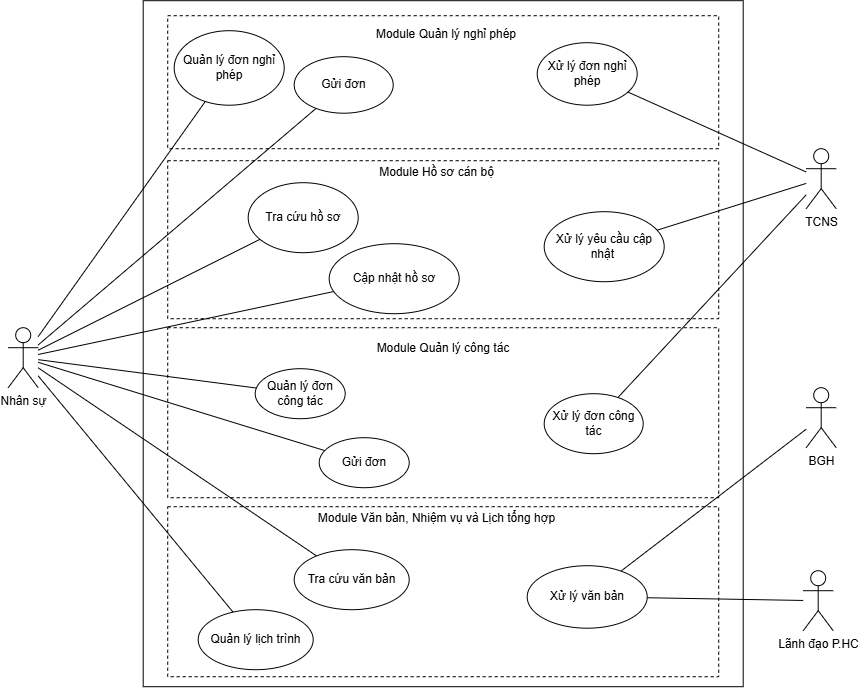
\includegraphics[width=0.95\linewidth]{image/usecase/UC-TQ.drawio.png}
    \caption{Sơ đồ Use Case tổng thể của MyHCMUT Mobile}
    \label{fig:system_usecase_diagram}
\end{figure}
% END SOURCE: Chapter4/section1.tex

\newpage

% BEGIN SOURCE: Chapter4/section2/index.tex
\section{Yêu cầu chức năng và đặc tả nghiệp vụ}
\label{sec:yeucau_chucnang}
\label{sec:yeucau_chucnang_modules}

Các yêu cầu chức năng được tổ chức theo bốn nhóm nghiệp vụ chính. Use case mô tả mục tiêu và tương tác của người dùng; biểu đồ hoạt động thể hiện các nhánh xử lý chính; biểu đồ tuần tự mô tả sự phối hợp giữa ứng dụng và các hệ thống liên quan.

Các luồng trong chương này mô tả hành vi nghiệp vụ cần hỗ trợ. Mức độ hiện thực và kết quả kiểm thử các luồng nghiệp vụ trên hệ thống tích hợp được trình bày tại Chương~6.

\begin{table}[H]
\centering
\small
\caption{Phạm vi đặc tả theo nhóm nghiệp vụ}
\label{tab:module_owner_scope}
\begin{tabularx}{\textwidth}{|L{4.2cm}|Y|}
\hline
\textbf{Nhóm nghiệp vụ} & \textbf{Phạm vi đặc tả trong chương} \\
\hline
Quản lý hồ sơ cá nhân & Tra cứu các danh mục thông tin lý lịch nhân sự; cập nhật trực tiếp các thông tin được phép hoặc gửi đề xuất kèm minh chứng đối với thông tin cần thẩm định; gửi phản hồi và tra cứu lịch sử xử lý. \\
\hline
Quản lý nghỉ phép & Tra cứu quỹ phép tham khảo, lập và gửi đơn nghỉ phép qua quy trình hướng dẫn, theo dõi và xử lý yêu cầu theo quy trình phê duyệt. \\
\hline
Quản lý công tác & Lập và gửi hồ sơ công tác qua biểu mẫu hướng dẫn 5 bước, kiểm tra xung đột thời gian, theo dõi và xử lý hồ sơ theo quy trình phê duyệt. \\
\hline
Văn phòng số, nhiệm vụ và lịch công tác & Tra cứu, phân công và xử lý văn bản đến; xem văn bản đi, nhiệm vụ và lịch tổng hợp; tạo/đăng ký cuộc họp theo quyền, điểm danh và báo vắng. \\
\hline
\end{tabularx}
\end{table}


% BEGIN SOURCE: Chapter4/section2/profile/index.tex
\subsection{Quản lý hồ sơ cá nhân}
\label{subsec:req_profile}
\label{subsec:module_profile}

\subsubsection{Mục tiêu và yêu cầu chức năng}

HRM quản lý dữ liệu hồ sơ chính thức; MyHCMUT Mobile cung cấp giao diện native để tra cứu, chỉnh sửa, phản hồi và xem lịch sử. Chính sách do HRM cung cấp xác định cách xử lý từng trường: cập nhật trực tiếp hoặc gửi đề xuất cần thẩm định. Hai loại trường có thể cùng xuất hiện trong một lần thao tác. Mobile dùng chính sách để dựng biểu mẫu; HRM kiểm tra lại quyền, dữ liệu và chính sách khi ghi nhận.

Thông tin được phân thành ba nhóm giao diện trong Bảng~\ref{tab:profile_groups}. Chuyên viên TCNS có quyền thẩm định đối chiếu nội dung đề xuất với dữ liệu hiện tại và minh chứng, sau đó xử lý từng nội dung được phân công.

\begin{table}[H]
\centering
\small
\caption{Phân nhóm danh mục thông tin hồ sơ nhân sự}
\label{tab:profile_groups}
\vspace{0.15cm}
\begin{tabularx}{\textwidth}{|L{4.2cm}|Y|}
\hline
\textbf{Nhóm giao diện} & \textbf{Các danh mục thông tin thành phần} \\
\hline
\textbf{Cá nhân và gia đình} & Thông tin cá nhân cơ bản; Địa chỉ cư trú (thường trú, tạm trú); Quan hệ gia đình (thân nhân, người phụ thuộc). \\
\hline
\textbf{Công tác và đào tạo} & Quá trình công tác / vị trí việc làm hiện tại; Trình độ học vấn, văn bằng chứng chỉ và quá trình đào tạo, bồi dưỡng chuyên môn. \\
\hline
\textbf{Chế độ và thông tin khác} & Quá trình lương và phụ cấp; Khen thưởng; Kỷ luật; Thông tin sức khỏe; Kê khai tài sản / thu nhập. \\
\hline
\end{tabularx}
\end{table}

\begin{table}[H]
\centering
\small
\caption{Yêu cầu chức năng nhóm quản lý hồ sơ cá nhân}
\label{tab:fr_profile}
\begin{tabularx}{\textwidth}{|L{1.8cm}|L{3.5cm}|L{2.5cm}|Y|}
\hline
\textbf{Mã FR} & \textbf{Chức năng} & \textbf{Tác nhân} & \textbf{Mô tả và ràng buộc nghiệp vụ} \\
\hline
FR-PRO-01 & Tra cứu hồ sơ & Nhân sự & Xem các danh mục thông tin lý lịch cá nhân do HRM cung cấp. \\
\hline
FR-PRO-02 & Cập nhật hồ sơ & Nhân sự & Chỉnh sửa bằng biểu mẫu native theo chính sách từng trường; HRM kiểm tra quyền và dữ liệu để cập nhật trực tiếp hoặc tiếp nhận đề xuất kèm minh chứng. \\
\hline
FR-PRO-03 & Thẩm định đề xuất & Chuyên viên TCNS & Đối với đề xuất cần thẩm định, xem xét thông tin sai khác, đối chiếu minh chứng và phê duyệt hoặc từ chối theo thẩm quyền. \\
\hline
FR-PRO-04 & Gửi phản hồi hồ sơ & Nhân sự & Gửi nội dung phản hồi kèm ít nhất một tài liệu minh chứng về danh mục hồ sơ; phản hồi không tự cập nhật dữ liệu chính thức. \\
\hline
FR-PRO-05 & Xem lịch sử hồ sơ & Nhân sự & Quan sát yêu cầu và nhật ký cập nhật; đối chiếu dữ liệu ban đầu với dữ liệu mới hoặc đề xuất theo từng trường, kèm trạng thái xử lý do HRM trả về. \\
\hline

\end{tabularx}
\end{table}

\subsubsection{Đặc tả Use Case}

UC-PRO-01 đến UC-PRO-05 lần lượt tương ứng FR-PRO-01 đến FR-PRO-05. Hình~\ref{fig:uc_profile} minh họa các nhánh nghiệp vụ; UC-PRO-05 bổ sung chức năng lịch sử.

\begin{figure}[H]
\centering
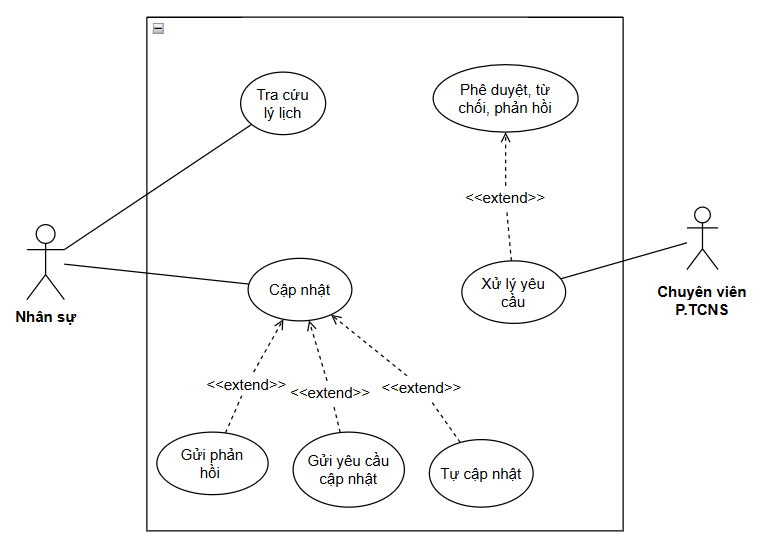
\includegraphics[width=\linewidth]{image/usecase/UC_PROFILE.png}
\caption{Sơ đồ Đặc tả Use case nhóm Quản lý hồ sơ cá nhân}
\label{fig:uc_profile}
\end{figure}

\usecasespec{
  id={UC-PRO-01},
  name={Tra cứu hồ sơ nhân sự},
  shortname={Tra cứu hồ sơ},
  actor={Nhân sự},
  desc={Cho phép nhân sự tra cứu các danh mục thông tin lý lịch cá nhân được cung cấp bởi hệ thống HRM.},
  pre={Nhân sự đã đăng nhập thành công vào ứng dụng MyHCMUT Mobile.},
  trigger={Người dùng chọn mục ``Hồ sơ cá nhân'' trên ứng dụng di động.},
  mainflow={
    1. Người dùng mở giao diện hồ sơ cá nhân trên ứng dụng. \newline
    2. Ứng dụng hiển thị thông tin tổng quan và ba nhóm giao diện chính. \newline
    3. Người dùng lựa chọn nhóm và danh mục thông tin cần xem. \newline
    4. Ứng dụng tải và hiển thị chi tiết các trường dữ liệu tương ứng từ hệ thống HRM.
  },
  altflow={
    - \textit{Luồng 2a (Làm mới dữ liệu):} Người dùng thực hiện làm mới để yêu cầu ứng dụng tải dữ liệu mới nhất từ hệ thống HRM.
  },
  exflow={
    - \textit{Ngoại lệ 4a (Lỗi kết nối):} Khi không thể tải dữ liệu từ hệ thống HRM, ứng dụng sử dụng dữ liệu hồ sơ đã lưu tạm trước đó nếu có và thông báo trạng thái kết nối cho người dùng. Nếu chưa có dữ liệu lưu tạm, ứng dụng thông báo không thể tải dữ liệu.
  },
  post={Người dùng xem được dữ liệu hồ sơ mới nhất tải được từ HRM hoặc dữ liệu đã lưu tạm gần nhất khi không thể kết nối.},
  label={tab:uc_pro_01}
}

\usecasespec{
  id={UC-PRO-02},
  name={Cập nhật hồ sơ cá nhân},
  shortname={Cập nhật hồ sơ},
  actor={Nhân sự},
  desc={Cho phép nhân sự cập nhật thông tin hồ sơ theo phạm vi quyền; HRM ghi nhận trực tiếp các thông tin được phép và tiếp nhận đề xuất đối với thông tin cần thẩm định.},
  pre={Nhân sự đã đăng nhập vào MyHCMUT Mobile và đang xem hồ sơ của bản thân.},
  trigger={Người dùng chọn chức năng cập nhật tại danh mục thông tin tương ứng.},
  mainflow={
    1. Người dùng chọn cập nhật thông tin hồ sơ. \newline
    2. Ứng dụng tải dữ liệu hiện tại và chính sách cập nhật từ HRM, sau đó mở biểu mẫu Flutter của danh mục được hỗ trợ. \newline
    3. Người dùng điều chỉnh các thông tin cần thay đổi và cung cấp tài liệu minh chứng đối với những nội dung yêu cầu minh chứng. \newline
    4. Ứng dụng kiểm tra dữ liệu đầu vào và minh chứng theo chính sách, chỉ gửi những trường thực sự thay đổi khi người dùng xác nhận. \newline
    5. HRM kiểm tra quyền, tính hợp lệ của dữ liệu và chính sách áp dụng cho từng trường thông tin. \newline
    6. Các trường được phép tự cập nhật được ghi nhận trực tiếp; các trường cần thẩm định được ghi nhận thành nội dung đề xuất chờ xử lý. \newline
    7. Hệ thống phản hồi kết quả để người dùng theo dõi thông tin hoặc trạng thái đề xuất tương ứng.
  },
  exflow={
    - \textit{Ngoại lệ 4a (Thiếu tài liệu minh chứng):} Khi thiếu tài liệu minh chứng đối với nội dung yêu cầu minh chứng, hệ thống thông báo để người dùng bổ sung trước khi tiếp nhận nội dung tương ứng. \newline
    - \textit{Ngoại lệ 4b (Mất kết nối):} Ứng dụng thông báo lỗi; không coi dữ liệu đang nhập là thay đổi đã được HRM lưu. Khi chưa xác định kết quả gửi, người dùng cần kiểm tra hồ sơ hoặc lịch sử trước khi gửi lại. \newline
    - \textit{Ngoại lệ 5a (Không đáp ứng điều kiện nghiệp vụ):} Khi tồn tại điều kiện nghiệp vụ không cho phép tiếp nhận thay đổi, hệ thống từ chối thao tác và phản hồi nguyên nhân cho người dùng.
  },
  post={Thông tin được phép đã được cập nhật vào hồ sơ; các thông tin cần thẩm định được ghi nhận thành đề xuất chờ xử lý.},
  label={tab:uc_pro_02}
}

\usecasespec{
  id={UC-PRO-03},
  name={Thẩm định thay đổi hồ sơ},
  shortname={Thẩm định thay đổi hồ sơ},
  actor={Chuyên viên Phòng Tổ chức Nhân sự có thẩm quyền},
  desc={Cho phép chuyên viên TCNS có thẩm quyền đối chiếu nội dung đề xuất với dữ liệu hiện tại và tài liệu minh chứng, sau đó xử lý các nội dung thay đổi theo phạm vi được phân công.},
  pre={Chuyên viên đã đăng nhập và tài khoản được phân quyền thẩm định hồ sơ nhân sự.},
  trigger={Chuyên viên mở danh sách các đề xuất cập nhật hồ sơ đang chờ xử lý.},
  mainflow={
    1. Chuyên viên mở danh sách đề xuất cập nhật hồ sơ chờ xử lý. \newline
    2. Chọn một đề xuất cụ thể để xem chi tiết. \newline
    3. Ứng dụng hiển thị thông tin hiện tại và nội dung đề xuất để chuyên viên đối chiếu, kèm tài liệu minh chứng tương ứng. \newline
    4. Chuyên viên lựa chọn phê duyệt hoặc từ chối đối với từng nội dung thay đổi theo phạm vi được cấp quyền. \newline
    5. Đối với thao tác từ chối, ứng dụng yêu cầu chuyên viên nhập lý do. \newline
    6. Hệ thống ghi nhận kết quả xử lý của từng nội dung. Khi toàn bộ nội dung thuộc đề xuất đã được xử lý, trạng thái của đề xuất được cập nhật tương ứng và các thay đổi được chấp thuận được phản ánh vào hồ sơ. \newline
    7. Kết quả xử lý được ghi nhận để người đề xuất theo dõi.
  },
  altflow={
    - \textit{Luồng 4a (Xử lý từng phần):} Một đề xuất có thể được xử lý từng phần; các nội dung đã được xử lý được ghi nhận kết quả trong khi các nội dung còn lại tiếp tục chờ xử lý.
  },
  exflow={
    - \textit{Ngoại lệ 4a (Trạng thái hoặc quyền xử lý thay đổi):} Khi thao tác không còn hợp lệ do trạng thái đề xuất đã thay đổi hoặc người dùng không còn quyền xử lý nội dung tương ứng, hệ thống từ chối thao tác và yêu cầu làm mới trạng thái hiện tại.
  },
  post={Kết quả xử lý của từng nội dung được ghi nhận; khi toàn bộ nội dung đã được xử lý, đề xuất đạt trạng thái kết thúc tương ứng và dữ liệu hồ sơ phản ánh các thay đổi đã được chấp thuận.},
  label={tab:uc_pro_03}
}

\usecasespec{
 id={UC-PRO-04}, name={Gửi phản hồi hồ sơ}, shortname={Gửi phản hồi}, actor={Nhân sự},
 desc={Ghi nhận phản hồi liên quan đến một danh mục hồ sơ bằng giao diện native.},
 pre={Người dùng đã đăng nhập và có quyền gửi phản hồi tại danh mục tương ứng.},
 trigger={Người dùng chọn gửi phản hồi trong menu thao tác hồ sơ.},
 mainflow={1. Ứng dụng mở biểu mẫu phản hồi của danh mục được chọn. \newline
 2. Người dùng nhập nội dung phản hồi và đính kèm ít nhất một tài liệu minh chứng. \newline
 3. Ứng dụng gửi nội dung theo hợp đồng API phản hồi của HRM. \newline
 4. HRM kiểm tra quyền và dữ liệu, ghi nhận phản hồi rồi trả kết quả. \newline
 5. Ứng dụng thông báo kết quả; người dùng theo dõi tại lịch sử hồ sơ.},
 exflow={- Thiếu nội dung hoặc minh chứng: yêu cầu bổ sung trước khi gửi. \newline
 - Dữ liệu không hợp lệ, quyền thay đổi hoặc lỗi kết nối: hiển thị lỗi; không thông báo gửi thành công khi backend chưa xác nhận.},
 post={Phản hồi hợp lệ được ghi nhận; dữ liệu hồ sơ chính thức không tự thay đổi chỉ vì đã gửi phản hồi.}, label={tab:uc_pro_04}
}
\usecasespec{
 id={UC-PRO-05}, name={Xem lịch sử hồ sơ}, shortname={Xem lịch sử}, actor={Nhân sự},
 desc={Tra cứu các yêu cầu, nội dung thay đổi và nhật ký mà HRM cho phép người dùng xem.},
 pre={Người dùng đã đăng nhập và được truy cập lịch sử hồ sơ tương ứng.},
 trigger={Người dùng chọn mục lịch sử hồ sơ.},
 mainflow={1. Ứng dụng yêu cầu lịch sử từ HRM. \newline
 2. HRM xác định phạm vi dữ liệu theo phiên và quyền, trả yêu cầu cùng nhật ký liên quan. \newline
 3. Ứng dụng trình bày hai nhóm yêu cầu và thay đổi đã ghi nhận, kèm thời điểm, trạng thái và thông tin xử lý được backend trả về. \newline
 4. Người dùng mở chi tiết để quan sát các trường khác nhau, đối chiếu dữ liệu ban đầu với dữ liệu mới hoặc nội dung đề xuất; xem lý do và minh chứng nếu có.},
 altflow={- Không có lịch sử: ứng dụng hiển thị trạng thái danh sách rỗng.},
 exflow={- Không thể tải hoặc không đủ quyền: thông báo lỗi, không diễn giải dữ liệu chưa tải là không có yêu cầu.},
 post={Người dùng xem được lịch sử do HRM cung cấp; thao tác này không thay đổi trạng thái yêu cầu.}, label={tab:uc_pro_05}
}

UC-PRO-05 sử dụng giá trị trước/sau do HRM trả về để đối chiếu từng trường có dữ liệu lịch sử; nội dung chờ duyệt hoặc bị từ chối chưa phải dữ liệu có hiệu lực. Phạm vi chỉnh sửa native gồm thông tin cá nhân, địa chỉ, ngân hàng/bảo hiểm, gia đình, công tác ngoài Trường, đào tạo và kê khai tài sản/thu nhập. Chính sách chỉnh sửa và minh chứng được áp dụng riêng theo danh mục, không mặc định mọi trường đều được sửa hoặc đều cần tệp.

\subsubsection{Biểu đồ hoạt động}

Hình~\ref{fig:act_profile_request} thể hiện cập nhật trực tiếp và thẩm định đề xuất theo từng nhóm trường; cả hai hướng có thể cùng xuất hiện trong một lần cập nhật.

\begin{figure}[H]
\centering
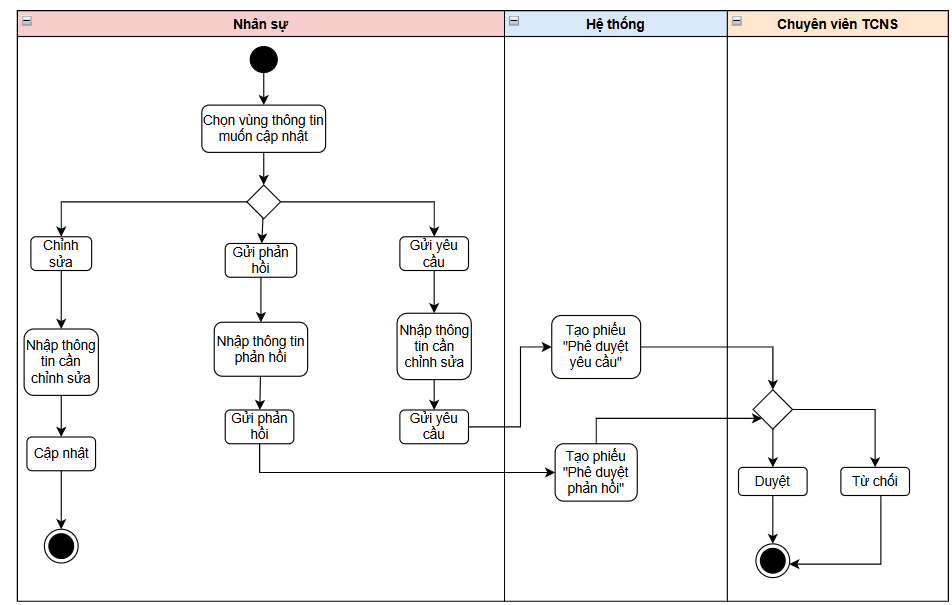
\includegraphics[width=\linewidth]{image/uml/profile_activity.png}
\caption{Biểu đồ hoạt động Quy trình cập nhật hồ sơ cá nhân}
\label{fig:act_profile_request}
\end{figure}

\subsubsection{Biểu đồ tuần tự}

Hình~\ref{fig:seq_profile_request} minh họa lấy dữ liệu/chính sách, gửi nội dung thay đổi và xử lý tại HRM. Hai nhánh cập nhật trực tiếp và đề xuất áp dụng theo trường. Hợp đồng API và truyền tệp được trình bày tại Chương~5.

\begin{figure}[H]
\centering
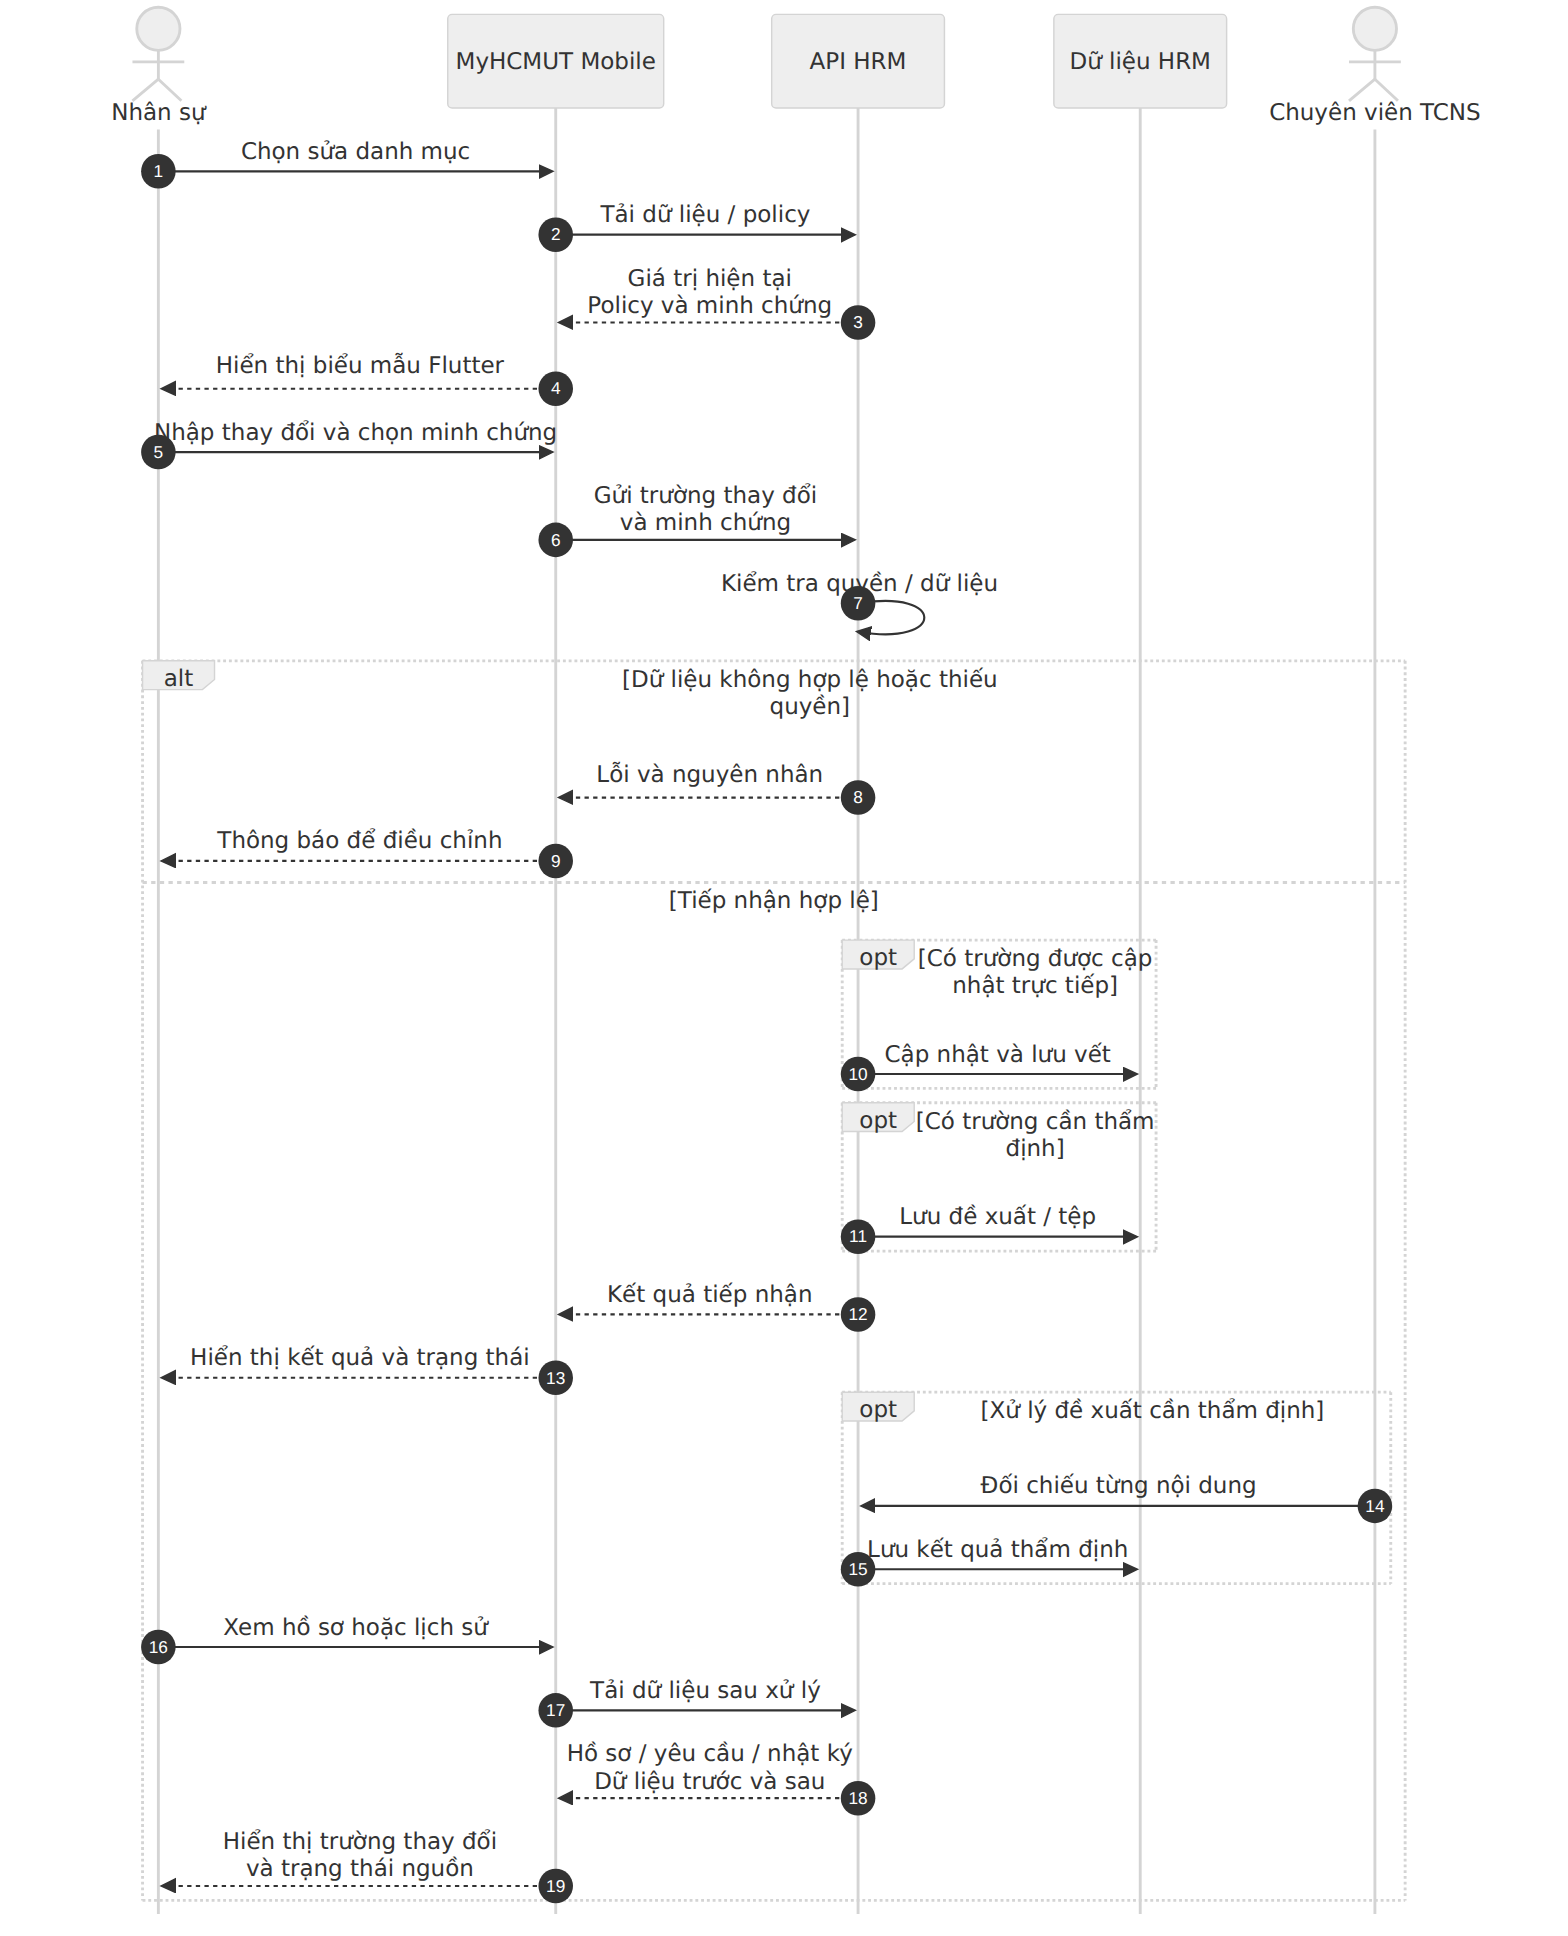
\includegraphics[width=\linewidth]{image/uml/seq_profile_request.png}
\caption{Biểu đồ tuần tự Cập nhật hồ sơ cá nhân}
\label{fig:seq_profile_request}
\end{figure}
% END SOURCE: Chapter4/section2/profile/index.tex


% BEGIN SOURCE: Chapter4/section2/leave/index.tex
\subsection{Quản lý nghỉ phép}
\label{subsec:req_leave}
\label{subsec:module_leave}

\subsubsection{Mục tiêu và yêu cầu chức năng}

Ứng dụng hỗ trợ tra cứu quỹ phép tham khảo, lập đơn theo biểu mẫu ba bước, theo dõi và xử lý theo thẩm quyền. Kiểm tra ngày, số dư và xung đột trên mobile hỗ trợ hoàn thiện dữ liệu; backend HRM thực hiện kiểm tra nghiệp vụ cuối cùng và xử lý việc chuyển trạng thái hồ sơ.

\begin{table}[H]
\centering
\small
\caption{Yêu cầu chức năng nhóm quản lý nghỉ phép}
\label{tab:fr_leave}
\begin{tabularx}{\textwidth}{|L{1.8cm}|L{3.5cm}|L{2.5cm}|Y|}
\hline
\textbf{Mã FR} & \textbf{Chức năng} & \textbf{Tác nhân} & \textbf{Mô tả và ràng buộc nghiệp vụ} \\
\hline
FR-LEV-01 & Tra cứu quỹ phép và đơn & Nhân sự & Xem số dư quỹ phép năm tham khảo, lọc danh sách đơn theo năm và trạng thái xử lý. \\
\hline
FR-LEV-02 & Lập và gửi đơn nghỉ phép & Nhân sự & Nhập liệu theo biểu mẫu 3 bước, đính kèm minh chứng, lưu nháp hoặc gửi duyệt khi đáp ứng điều kiện nghiệp vụ. \\
\hline
FR-LEV-03 & Quản lý đơn đã tạo & Nhân sự & Chỉnh sửa hoặc xóa đơn ở trạng thái Nháp; chỉnh sửa và gửi lại đơn Bị trả lại. Đơn đã gửi không mặc định có thao tác thu hồi cho người lập. \\
\hline
FR-LEV-04 & Phê duyệt theo thẩm quyền & Cấp phê duyệt & Xem xét nội dung, minh chứng và phê duyệt, từ chối hoặc trả lại đơn theo thẩm quyền được phân công. \\
\hline
\end{tabularx}
\end{table}

Trong quy trình hiện thực, thao tác lưu giữ đơn ở trạng thái Nháp, còn thao tác gửi mới chuyển đơn sang bước chờ duyệt. Quyền thu hồi của người có thẩm quyền thuộc luồng xử lý riêng, không đồng nhất với quyền xóa đơn Nháp của người lập.

\subsubsection{Đặc tả Use Case}

UC-LEV-01 cụ thể hóa FR-LEV-01 và FR-LEV-03; UC-LEV-02 gắn với FR-LEV-02, còn UC-LEV-03 gắn với FR-LEV-04. Hình~\ref{fig:uc_leave} thể hiện các nhóm thao tác tương ứng.

\begin{figure}[H]
\centering
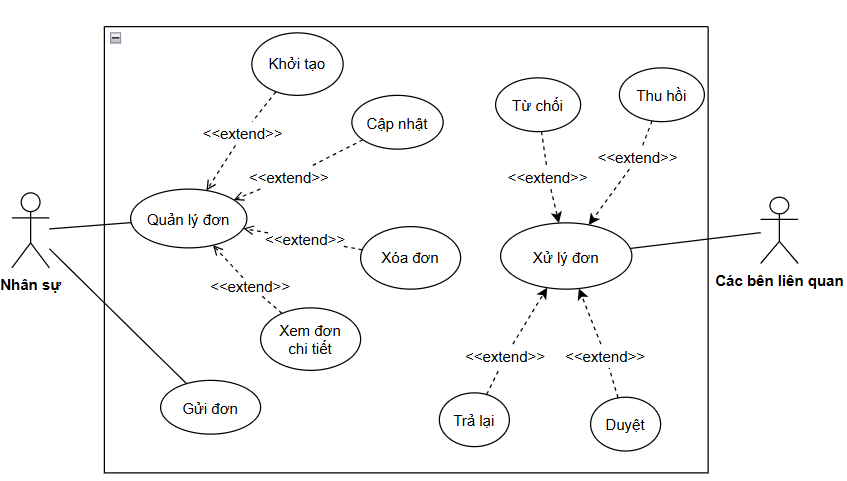
\includegraphics[width=\linewidth]{image/usecase/UC_LEAVE.png}
\caption{Sơ đồ Đặc tả Use case nhóm Quản lý nghỉ phép}
\label{fig:uc_leave}
\end{figure}

\usecasespec{
  id={UC-LEV-01},
  name={Quản lý đơn nghỉ phép cá nhân},
  shortname={Quản lý đơn cá nhân},
  actor={Nhân sự},
  desc={Cho phép nhân sự theo dõi số dư quỹ phép năm, tra cứu danh sách đơn và tiến trình duyệt; chỉnh sửa hoặc xóa đơn Nháp, chỉnh sửa và gửi lại đơn Bị trả lại.},
  pre={Nhân sự đã đăng nhập thành công vào ứng dụng MyHCMUT Mobile.},
  trigger={Người dùng chọn chức năng ``Nghỉ phép'' trên màn hình chính.},
  mainflow={
    1. Người dùng mở mục ``Nghỉ phép'' để xem số dư quỹ phép tham khảo và danh sách đơn đã lập. \newline
    2. Người dùng lọc danh sách hoặc chọn một đơn để xem trạng thái và tiến trình xử lý. \newline
    3. Với đơn Nháp, người dùng có thể tiếp tục chỉnh sửa hoặc xóa đơn. \newline
    4. HRM kiểm tra người lập và trạng thái đơn trước khi ghi nhận thao tác hợp lệ.
  },
  altflow={
    - \textit{Luồng 3a (Sửa đơn bị trả lại):} Với đơn ở trạng thái Bị trả lại, người dùng chọn chỉnh sửa để bổ sung thông tin và gửi lại. \newline
    - \textit{Luồng 3b (Theo dõi đơn đã gửi):} Với đơn đang chờ duyệt, người dùng xem trạng thái và lịch sử xử lý; ứng dụng không mặc định cung cấp thao tác thu hồi cho người lập.
  },
  exflow={
    - \textit{Ngoại lệ 4a (Trạng thái đã thay đổi):} Nếu đơn không còn ở trạng thái cho phép chỉnh sửa hoặc xóa, HRM từ chối thao tác và ứng dụng cập nhật trạng thái mới.
  },
  post={Nhân sự nắm bắt thông tin quỹ phép và trạng thái các đơn; những thay đổi hợp lệ đối với đơn Nháp hoặc đơn Bị trả lại được ghi nhận trên HRM.},
  label={tab:uc_lev_01}
}

\usecasespec{
  id={UC-LEV-02},
  name={Lập và gửi đơn nghỉ phép},
  shortname={Lập và gửi đơn nghỉ phép},
  actor={Nhân sự},
  desc={Cho phép nhân sự lập mới đơn nghỉ phép qua quy trình hướng dẫn 3 bước, kiểm tra thời gian và số dư phép, đính kèm minh chứng và gửi duyệt.},
  pre={Nhân sự đã đăng nhập vào hệ thống và có quyền lập đơn nghỉ phép.},
  trigger={Người dùng nhấn nút tạo mới đơn nghỉ phép trên giao diện ứng dụng.},
  mainflow={
    1. Người dùng chọn tạo mới đơn nghỉ phép; ứng dụng kiểm tra ngày đăng ký có hợp lệ trước khi yêu cầu tạo nháp. \newline
    2. Khi ngày đăng ký hợp lệ, hệ thống khởi tạo bản ghi nháp. \newline
    3. Người dùng nhập thông tin nghỉ phép và đính kèm minh chứng khi được yêu cầu. \newline
    4. Người dùng rà soát thông tin và gửi đơn. \newline
    5. HRM kiểm tra các điều kiện nghiệp vụ và tiếp nhận đơn hợp lệ vào quy trình chờ duyệt.
  },
  altflow={
    - \textit{Luồng 3a (Lưu nháp):} Người dùng chọn lưu nháp tại bất kỳ bước nào để tiếp tục hoàn thiện sau. \newline
    - \textit{Luồng 3b (Thoát biểu mẫu):} Người dùng xác nhận thoát; dữ liệu chưa lưu trên ứng dụng bị bỏ. Bản ghi nháp đã tạo trên HRM vẫn tồn tại, có thể mở lại hoặc xóa bằng thao tác riêng.
  },
  exflow={
    - \textit{Ngoại lệ 1a (Ngày đăng ký không hợp lệ):} Ứng dụng thông báo nguyên nhân và không tạo bản ghi nháp. \newline
    - \textit{Ngoại lệ 3a (Xung đột lịch trình):} Khoảng thời gian nghỉ trùng lặp với kế hoạch công tác hoặc đơn khác $\rightarrow$ hệ thống cảnh báo và yêu cầu điều chỉnh. \newline
    - \textit{Ngoại lệ 3b (Vượt số dư quỹ phép):} Số ngày đăng ký vượt quá số dư phép năm còn lại $\rightarrow$ hệ thống cảnh báo để người dùng điều chỉnh. \newline
    - \textit{Ngoại lệ 3c (Quá hạn đăng ký):} Khi kiểm tra thời hạn xác định không thể tạo đơn nghỉ phép thông thường, ứng dụng thông báo nguyên nhân và điều hướng người dùng đến điểm truy cập phân hệ Giải trình. Việc lập và xử lý Giải trình không thuộc phạm vi hiện thực của use case này.
  },
  post={Khi gửi thành công, đơn được ghi nhận ở bước chờ duyệt và phát sinh thông báo theo quy trình. Nếu chỉ lưu hoặc thoát sau khi tạo nháp, đơn vẫn ở trạng thái Nháp.},
  label={tab:uc_lev_02}
}

\usecasespec{
  id={UC-LEV-03},
  name={Xử lý đơn nghỉ phép},
  shortname={Xử lý đơn nghỉ phép},
  actor={Lãnh đạo Đơn vị, Chuyên viên Phòng Tổ chức Nhân sự, Ban Giám hiệu},
  desc={Cho phép người có thẩm quyền thẩm định nội dung đơn, kiểm tra tài liệu minh chứng và thực hiện phê duyệt, từ chối hoặc yêu cầu bổ sung thông tin.},
  pre={Người duyệt đã đăng nhập và đơn đang ở bước thuộc thẩm quyền xử lý của tài khoản.},
  trigger={Người duyệt mở danh sách đơn chờ xử lý từ ứng dụng hoặc qua thông báo nhắc việc.},
  mainflow={
    1. Người duyệt mở danh sách đơn nghỉ phép chờ xử lý thuộc thẩm quyền phân công. \newline
    2. Chọn xem chi tiết một đơn để kiểm tra nội dung và minh chứng liên quan. \newline
    3. Người duyệt lựa chọn hành động: \textit{Phê duyệt}, \textit{Từ chối} hoặc \textit{Trả lại}. \newline
    4. HRM kiểm tra quyền và trạng thái đơn hiện tại, rồi ghi nhận kết quả xử lý hoặc chuyển đơn sang bước tiếp theo. \newline
    5. Hệ thống thông báo kết quả cho nhân sự lập đơn; số dư phép được cập nhật khi đơn hoàn tất theo quy tắc nghiệp vụ.
  },
  altflow={
    - \textit{Luồng 3a (Xử lý đồng loạt):} Người duyệt chọn nhiều đơn hợp lệ trên danh sách và thực hiện phê duyệt hàng loạt. \newline
    - \textit{Luồng 3b (Trả lại yêu cầu chỉnh sửa):} Người duyệt chọn ``Trả lại'' kèm ý kiến yêu cầu $\rightarrow$ đơn chuyển sang trạng thái Bị trả lại để nhân sự hoàn thiện.
  },
  exflow={
    - \textit{Ngoại lệ 3a (Từ chối đơn):} Người duyệt bắt buộc nhập lý do từ chối trước khi hệ thống ghi nhận kết quả. \newline
    - \textit{Ngoại lệ 4a (Trạng thái không phù hợp):} Khi HRM xác định đơn không còn ở bước cho phép xử lý, thao tác bị từ chối và người dùng cần tải lại dữ liệu. Kiểm tra này không được xem là bảo đảm chống mọi thao tác phê duyệt đồng thời.
  },
  post={Đơn được chuyển sang bước tiếp theo, trả lại hoặc kết thúc theo quyết định được HRM ghi nhận; dữ liệu nghỉ phép được cập nhật khi duyệt bước cuối theo quy trình.},
  label={tab:uc_lev_03}
}

\subsubsection{Biểu đồ hoạt động}

Hình~\ref{fig:act_leave_submit} mô tả lập đơn và luân chuyển phê duyệt. Khi quá hạn, ứng dụng thông báo và điều hướng đến điểm truy cập Giải trình; quy trình Giải trình nằm ngoài phạm vi use case nghỉ phép hiện tại.

\begin{figure}[H]
\centering
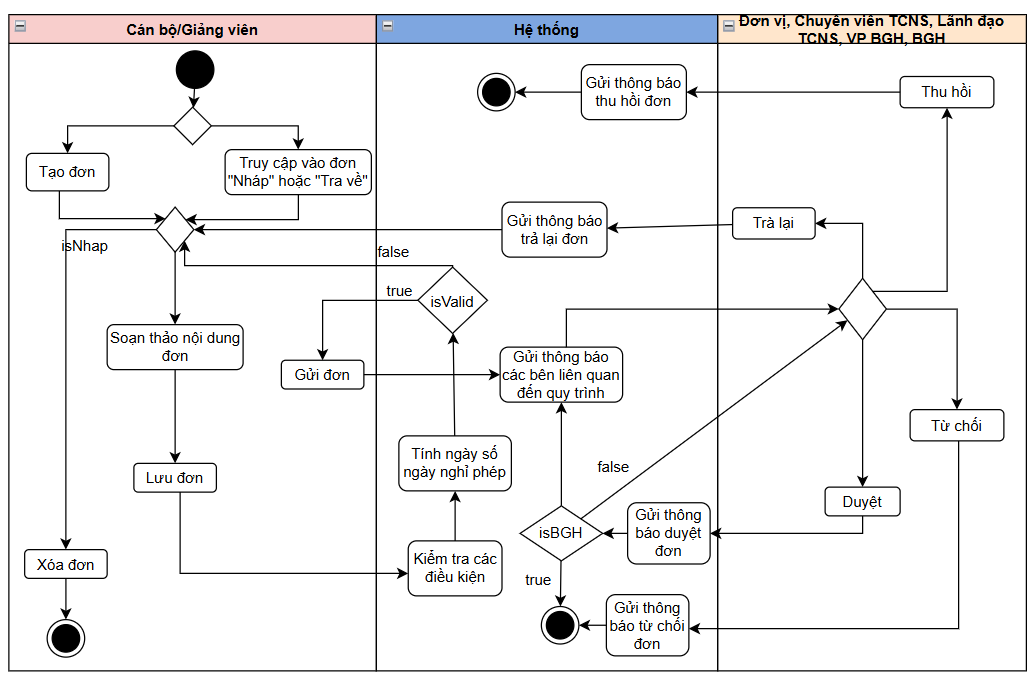
\includegraphics[width=\linewidth]{image/uml/leave_activity.png}
\caption{Biểu đồ hoạt động Quy trình nghỉ phép}
\label{fig:act_leave_submit}
\end{figure}

\subsubsection{Biểu đồ tuần tự}
Hình~\ref{fig:seq_leave_submit} minh họa UC-LEV-02: khởi tạo nháp, hoàn thiện dữ liệu và gửi vào quy trình chờ duyệt.

\begin{figure}[H]
\centering
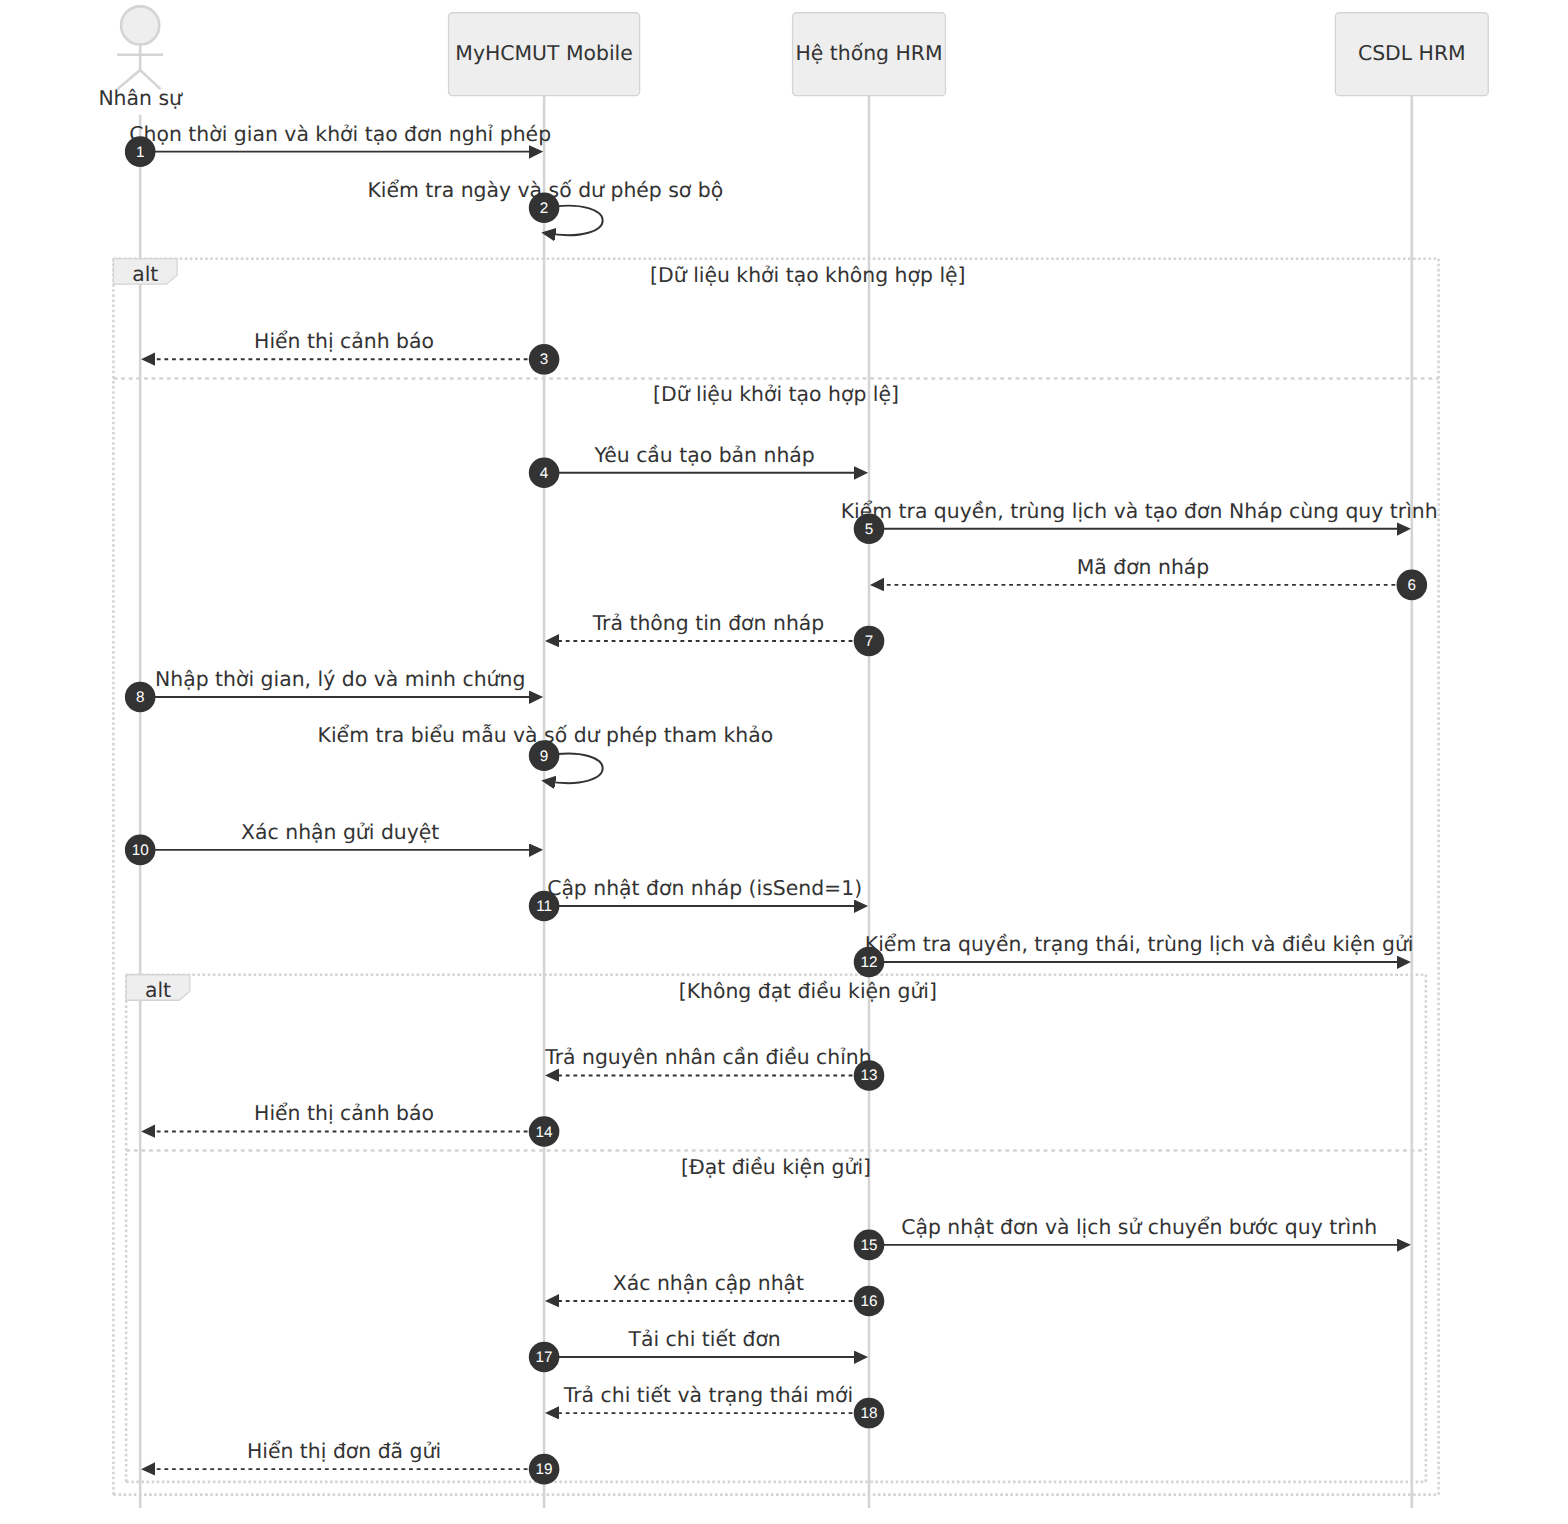
\includegraphics[width=\linewidth]{image/uml/seq_leave_submit.png}
\caption{Biểu đồ tuần tự Gửi yêu cầu nghỉ phép}
\label{fig:seq_leave_submit}
\end{figure}
% END SOURCE: Chapter4/section2/leave/index.tex


% BEGIN SOURCE: Chapter4/section2/hrm/business_trip.tex
\subsection{Phân hệ quản lý công tác}
\label{subsec:business_trip}

\subsubsection{Mục tiêu và yêu cầu chức năng}

Ứng dụng hỗ trợ lập, gửi và theo dõi phiếu công tác; người dùng có thẩm quyền thực hiện các thao tác xử lý theo quy trình của HRM. Các điều kiện và bước phê duyệt phụ thuộc vào thông tin chuyến công tác và quyền của người xử lý.

Việc nộp báo cáo kết quả sau chuyến công tác chưa thuộc phạm vi biểu mẫu trên ứng dụng di động.

\begin{table}[H]
\centering
\small
\caption{Yêu cầu chức năng nhóm quản lý công tác}
\label{tab:fr_business_trip}
\begin{tabularx}{\textwidth}{|L{1.8cm}|L{3.5cm}|L{2.5cm}|Y|}
\hline
\textbf{Mã FR} & \textbf{Chức năng} & \textbf{Tác nhân} & \textbf{Mô tả và ràng buộc nghiệp vụ} \\
\hline
FR-BTR-01 & Tra cứu đơn & Nhân sự & Xem danh sách đơn công tác cá nhân, lọc theo trạng thái và xem chi tiết tiến trình duyệt. \\
\hline
FR-BTR-02 & Tạo và gửi đơn & Nhân sự & Tạo phiếu đăng ký công tác, điền thông tin và gửi cho các bên liên quan phê duyệt. \\
\hline
FR-BTR-03 & Quản lý nháp và điều chỉnh & Nhân sự & Chỉnh sửa hoặc xóa phiếu Nháp; chỉnh sửa và gửi lại phiếu Bị trả lại. Người lập không tự thu hồi phiếu đã gửi. \\
\hline
FR-BTR-04 & Xử lý đơn & Các bên liên quan & Xem xét thông tin đơn đăng ký, minh chứng và thực hiện các thao tác như: phê duyệt, từ chối hoặc trả lại đơn theo thẩm quyền. \\
\hline
FR-BTR-05 & Thu hồi đơn & Nhân sự TCNS/Văn phòng BGH có quyền & Thu hồi theo quyền nghiệp vụ và điều kiện vai trò hoặc đơn vị do HRM kiểm tra; người lập không tự có quyền thu hồi. \\
\hline
\end{tabularx}
\end{table}

\subsubsection{Đặc tả Use Case}

FR-BTR-02 gắn với UC-BT-01/02; FR-BTR-03 gắn với UC-BT-01/03; FR-BTR-04/05 lần lượt gắn với UC-BT-04/05. FR-BTR-01 được cụ thể hóa qua tra cứu danh sách, chi tiết và theo dõi sau khi gửi.

\begin{figure}[H]
    \centering
    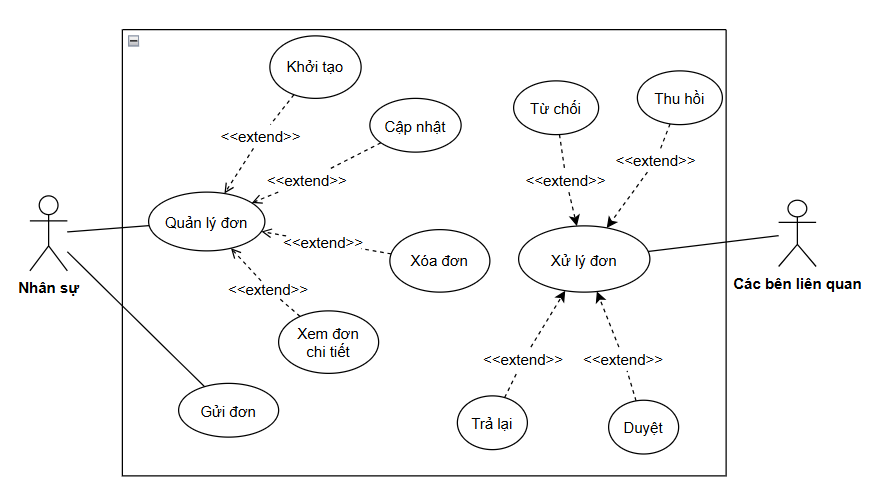
\includegraphics[width=\linewidth]{image/usecase/UC_BT.png}
    \caption{Sơ đồ use-case quản lý công tác}
    \label{fig:BT_UC}
\end{figure}

\usecasespec{
    id={UC-BT-01},
    name={Soạn thảo đơn đăng ký công tác},
    actor={Nhân sự},
    pre={Đã đăng nhập vào ứng dụng và tài khoản có quyền tạo đơn đăng ký công tác.},
    trigger={Người dùng chọn biểu tượng tạo mới đơn đăng ký công tác trên ứng dụng.},
    mainflow={
            1. Người dùng chọn ngày và loại công tác; HRM khởi tạo phiếu ở trạng thái Nháp (\texttt{NHAP}). \newline
            2. Người dùng hoàn thiện biểu mẫu năm bước: thời gian, hình thức trong nước/nước ngoài, cá nhân/đoàn, địa điểm, kinh phí, thành phần và minh chứng theo yêu cầu. \newline
            3. Người dùng nhấn nút "Lưu" đơn đăng ký công tác. \newline
            4. Hệ thống lưu lại thông tin đã nhập và đơn có trạng thái là "Nháp". \newline
        },
    altflow={
            1.1. Chọn đơn đăng ký công tác từ danh sách các đơn đã tạo có trạng thái là "Nháp" hoặc "Trả lại", hệ thống hiển thị thông tin chi tiết của đơn. Thực hiện tiếp bước 2. \newline
        },
    exflow={- Thiếu thông tin bắt buộc hoặc địa điểm không phù hợp: yêu cầu bổ sung trước khi tiếp tục. \newline
 - Thoát biểu mẫu: thay đổi chưa lưu bị bỏ; phiếu nháp đã tạo trên HRM vẫn có thể được mở lại hoặc xóa bằng thao tác riêng.},
    post={Thông tin đã lưu được ghi nhận; phiếu giữ trạng thái Nháp (\texttt{NHAP}) hoặc Trả lại (\texttt{TRA\_LAI}) đến khi được gửi hợp lệ.},
    label={tab:uc_bt_01}
}

\usecasespec{
    id={UC-BT-02},
    name={Gửi đơn đăng ký công tác},
    actor={Nhân sự},
    pre={Đã đăng nhập, có quyền gửi phiếu của bản thân và phiếu ở trạng thái Nháp hoặc Trả lại.},
    trigger={Người dùng mở phiếu Nháp hoặc Trả lại đã hoàn thiện thông tin},
    mainflow={
            1. Người dùng nhấn nút gửi đơn đăng ký công tác. \newline
            2. Hệ thống kiểm tra tính hợp lệ của thông tin nhập vào. \newline
            3. Hệ thống kiểm tra lịch trình cá nhân để rà soát xem có trùng lịch với các hoạt động khác không. \newline
            4. Hệ thống tạo quy trình phê duyệt tương ứng với thông tin của đơn đăng ký công tác và thêm vào lịch cá nhân của các thành viên tham gia. \newline
            5. Hệ thống gửi đơn đăng ký công tác đến các bên liên quan để thẩm định và phê duyệt. \newline
            6. Hệ thống ghi nhận khoảng thời gian công tác trong lịch cá nhân phục vụ kiểm tra xung đột và phát sinh thông báo theo quy trình. \newline
            7. Người dùng truy cập đơn đăng ký công tác để xem thông tin chi tiết, trạng thái phê duyệt, lịch sử thao tác.
        },
    exflow={
            2.1. Tại bước 2, nếu thông tin nhập vào không hợp lệ, hệ thống thông báo lỗi và yêu cầu người dùng chỉnh sửa. \newline
            3.1. Tại bước 3, nếu có trùng lịch trình cá nhân, hệ thống thông báo lỗi và yêu cầu người dùng chỉnh sửa lại thời gian công tác. \newline
        },
    post={Đơn đăng ký công tác được gửi đến các bên liên quan để thẩm định và phê duyệt.},
    label={tab:uc_bt_02}
}

\usecasespec{
    id={UC-BT-03},
    name={Xóa đơn đăng ký công tác},
    actor={Nhân sự},
    pre={Đã đăng nhập vào ứng dụng, là người lập đơn và đơn đang ở trạng thái Nháp.},
    trigger={Người dùng truy cập vào danh sách đơn đăng ký công tác.},
    mainflow={
            1. Người dùng chọn đơn đăng ký công tác có trạng thái là "Nháp" để xóa. \newline
            2. Người dùng nhấn nút "Xóa" để xóa đơn đăng ký công tác. \newline
            3. Hệ thống hiển thị hộp thoại xác nhận xóa đơn đăng ký công tác. \newline
            4. Người dùng xác nhận xóa đơn đăng ký công tác. \newline
            5. Hệ thống kiểm tra đơn vẫn ở trạng thái Nháp, sau đó xóa đơn đăng ký công tác.
        },
    exflow={
            5.1. Nếu đơn đã được gửi hoặc thay đổi trạng thái, hệ thống từ chối xóa và giữ nguyên dữ liệu.
        },
    post={Chỉ đơn Nháp hợp lệ được xóa khỏi hệ thống.},
    label={tab:uc_bt_03}
}

\usecasespec{
    id={UC-BT-04},
    name={Phê duyệt đơn đăng ký công tác},
    goal={Cho phép nhân sự có thẩm quyền tại từng cột mốc xem xét và đưa ra quyết định (Duyệt / Trả lại / Từ chối) đối với phiếu công tác đã được gửi, đưa phiếu đi qua chuỗi các cấp thẩm định phù hợp với loại công tác cho đến khi được Ban Giám hiệu phê duyệt chính thức hoặc bị chấm dứt.},
    actor={Lãnh đạo đơn vị, Lãnh đạo Phòng KH\&CN, Chuyên viên/ Lãnh đạo TCNS, Văn phòng Ban Giám hiệu, Ban Giám hiệu},
    pre={
            - Đơn đã được gửi và đang ở một trong các bước duyệt: \texttt{Lãnh đạo đơn vị}, \texttt{Lãnh đạo KHCN}, \texttt{Chuyên viên TCNS}, \texttt{Lãnh đạo TCNS}, \texttt{Chuyên viên BGH}, \texttt{BGH}. \newline
            - Người thực hiện có thẩm quyền duyệt tại đúng bước hiện tại của phiếu
        },
    trigger={Người duyệt mở phiếu đang chờ tại bước của mình và chọn một trong ba hành động: Duyệt, Trả lại, Từ chối.},
    mainflow={
            1. Người có thẩm quyền mở phiếu đang chờ tại bước được phân công. \newline
            2. Người duyệt xem xét thông tin chuyến đi, thời gian vắng mặt, phương án phân công thay thế. \newline
            3. Người duyệt chọn "Duyệt". \newline
            4. HRM kiểm tra quyền, bước xử lý và dữ liệu, ghi nhận quyết định và nhật ký quy trình. \newline
            5. Hệ thống gửi thông báo đến nhân sự có thẩm quyền duyệt ở bước kế tiếp. \newline
        },
    altflow={
            5.1. Tại bước 5, nếu phiếu đang ở bước duyệt cuối cùng (\texttt{BGH}), hệ thống chuyển phiếu sang trạng thái \texttt{Kết thúc}. \newline
            A2 — Trả lại phiếu: \newline
            3.2. Người duyệt chọn "Trả lại" và nhập ghi chú yêu cầu chỉnh sửa. \newline
            4.2. Hệ thống sẽ trả lại phiếu cho người nộp và mở lại quyền chỉnh sửa cho người nộp. \newline
            5.2. Hệ thống gửi thông báo kèm ghi chú cho người nộp. \newline
            A3 — Từ chối phiếu: \newline
            3.3. Người duyệt chọn "Từ chối" và nhập ghi chú lý do từ chối. \newline
            4.3. Hệ thống cập nhật trạng thái phiếu thành \texttt{Từ chối}. \newline
            5.3. HRM xóa các khoảng thời gian công tác gắn với phiếu trong lịch cá nhân của các thành viên. \newline
            6.3. Hệ thống thông báo cho người nộp và mọi thành viên liên quan. \newline
        },
    post={Đơn chuyển sang trạng thái mới thành công.},
    label={tab:uc_bt_04}
}

\usecasespec{
    id={UC-BT-05},
    name={Thu hồi đơn đăng ký công tác},
    actor={Nhân sự TCNS hoặc Văn phòng BGH được cấp quyền thu hồi},
    pre={Đã đăng nhập, có quyền xử lý công tác và đáp ứng điều kiện nhân sự thuộc TCNS hoặc vai trò Văn phòng BGH theo HRM.},
    trigger={Người dùng truy cập vào danh sách đơn đăng ký công tác.},
    mainflow={
            1. Người có quyền chọn phiếu đăng ký cần thu hồi và xem thông tin hiện tại. \newline
            2. Người dùng nhấn nút "Thu hồi" để thu hồi đơn đăng ký công tác. \newline
            3. Hệ thống hiển thị hộp thoại xác nhận thu hồi đơn đăng ký công tác. \newline
            4. Người dùng xác nhận thu hồi đơn đăng ký công tác. \newline
            5. HRM kiểm tra quyền và điều kiện vai trò/đơn vị; cập nhật phiếu thành Đã thu hồi (\texttt{THU\_HOI}), xóa dữ liệu lịch cá nhân và quá trình công tác gắn với phiếu. \newline
            6. Hệ thống thông báo cho người nộp và mọi thành viên liên quan về việc thu hồi phiếu.
        },
    exflow={- Không đủ quyền, không đáp ứng điều kiện vai trò/đơn vị hoặc phiếu không tồn tại: HRM từ chối thao tác.},
    post={Khi được HRM chấp nhận, phiếu chuyển sang Đã thu hồi (\texttt{THU\_HOI}); dữ liệu liên quan được xử lý theo quy trình.},
    label={tab:uc_bt_05}
}

\subsubsection{Biểu đồ hoạt động}
\begin{figure}[H]
    \centering
    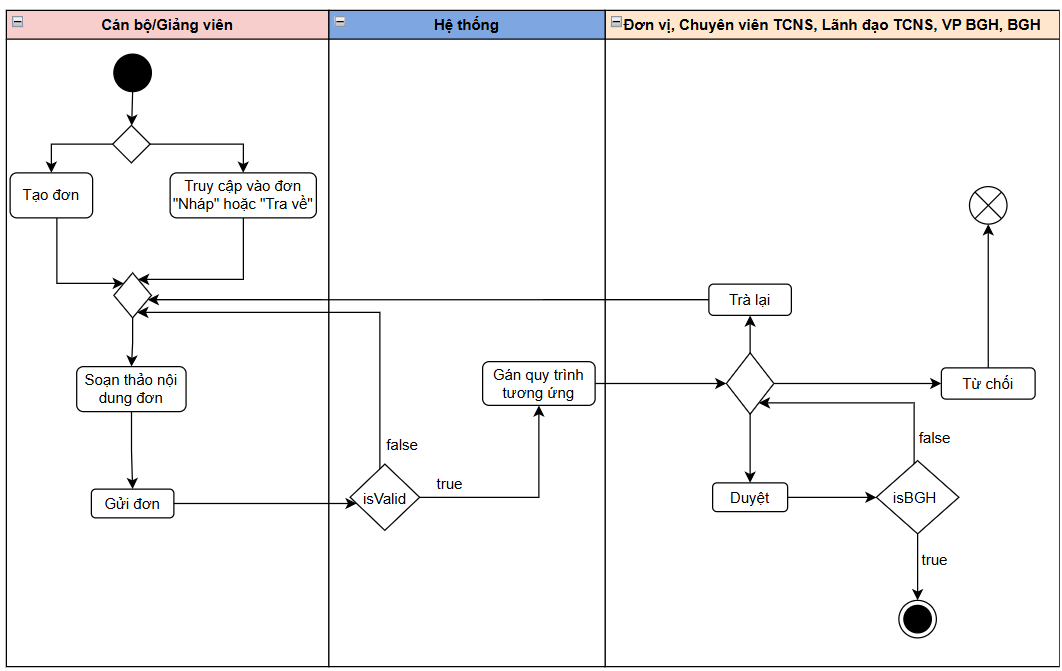
\includegraphics[width=\linewidth]{image/uml/bt_activity.png}
    \caption{Sơ đồ hoạt động quản lý công tác}
    \label{fig:BT_AC}
\end{figure}

\subsubsection{Biểu đồ tuần tự}
\begin{figure}[H]
    \centering
    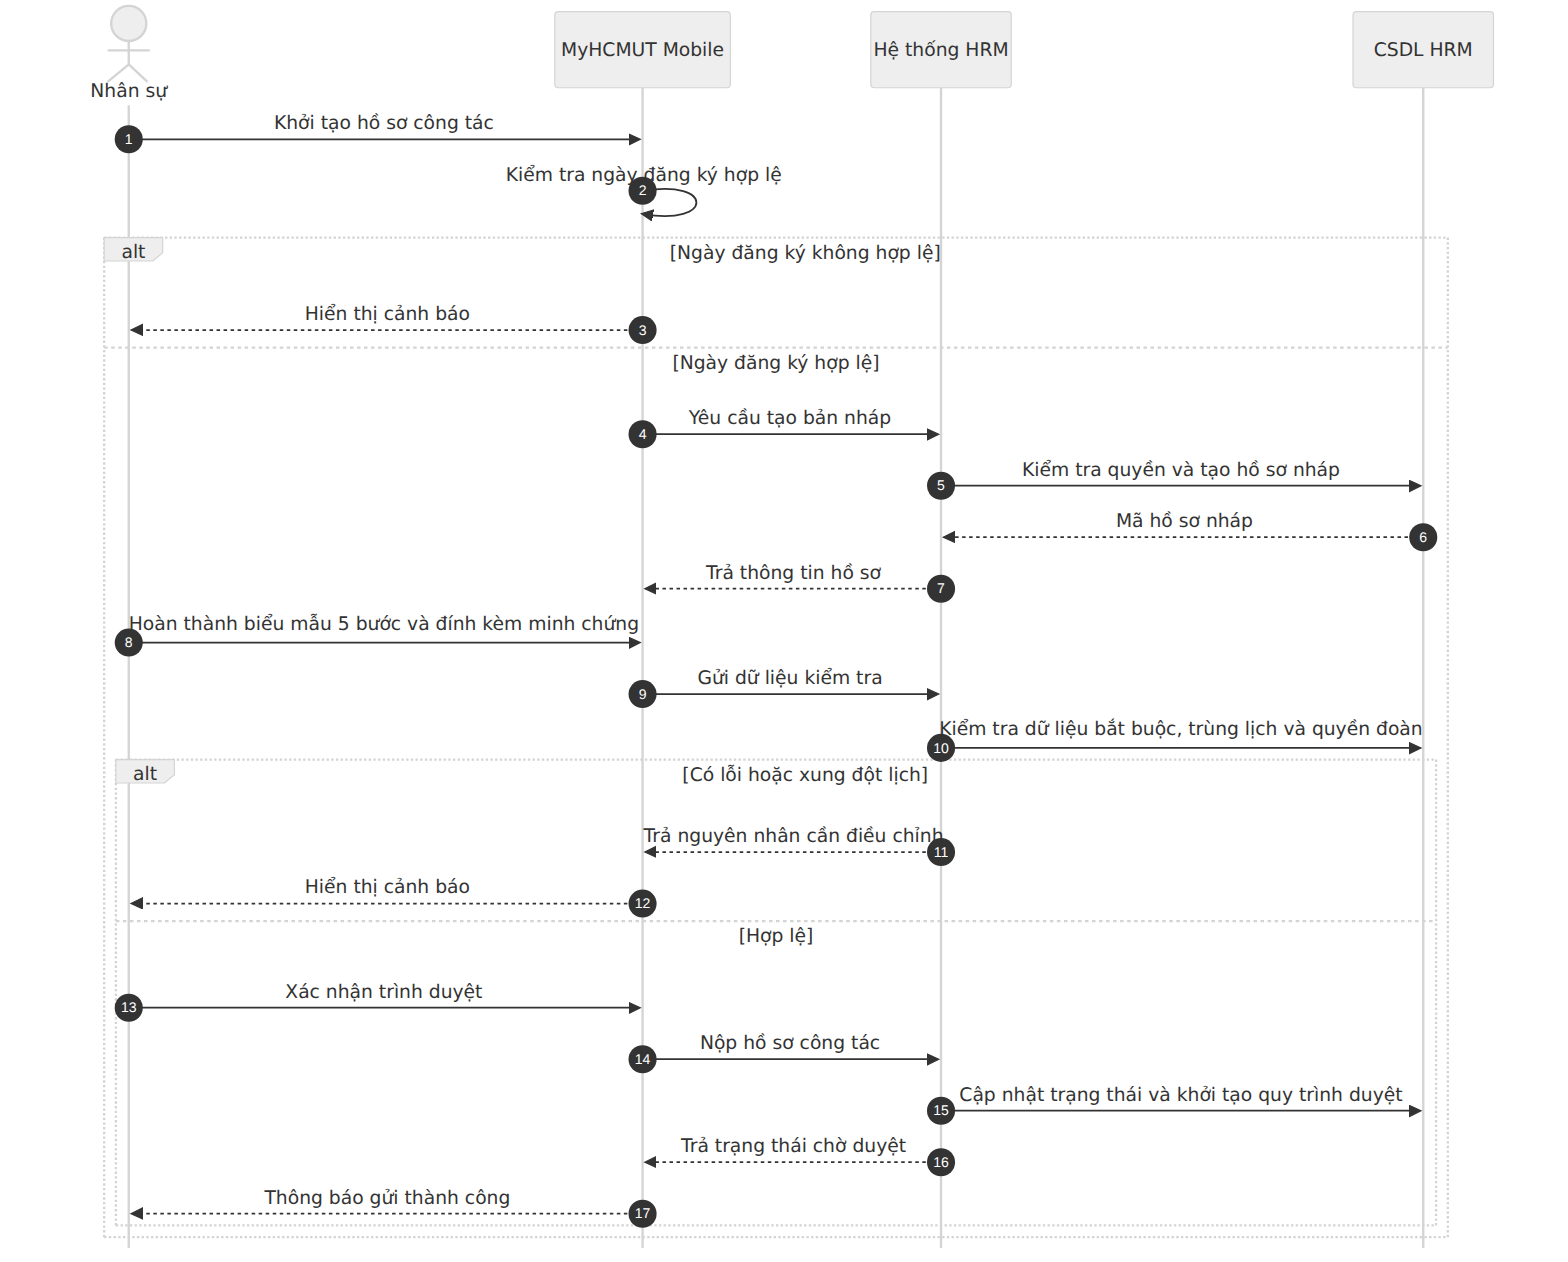
\includegraphics[width=\linewidth]{image/uml/seq_trip_submit.png}
    \caption{Sơ đồ tuần tự quản lý công tác}
    \label{fig:BT_SEQ}
\end{figure}
% END SOURCE: Chapter4/section2/hrm/business_trip.tex


% BEGIN SOURCE: Chapter4/section2/ioffice_schedule/index.tex
\subsection{Văn phòng số, nhiệm vụ và lịch công tác}
\label{subsec:module_ioffice}
\label{subsec:req_ioffice}
\label{subsec:req_schedule}

\subsubsection{Mục tiêu và yêu cầu chức năng}

Ứng dụng cung cấp chức năng tra cứu, phân công và xử lý văn bản đến, xem văn bản đi và theo dõi nhiệm vụ từ iOffice. Phân công trên mobile gắn với phiếu giải quyết văn bản đến; tạo hoặc phân công nhiệm vụ độc lập và nộp báo cáo tiến độ nằm ngoài phạm vi mobile.

Lịch tổng hợp (\textit{Unified Calendar}) kết hợp lịch họp iOffice với lịch nghỉ phép và công tác từ HRM, giúp người dùng theo dõi các loại lịch liên quan trên một giao diện. Dữ liệu gốc và thẩm quyền xử lý vẫn thuộc từng hệ thống nguồn.

Người dùng có quyền sử dụng lịch có thể ghi nhận có mặt, hoàn tác hoặc báo vắng trong cửa sổ thời gian được iOffice cho phép. Có phân công thì trạng thái gắn với dòng phân công; không có phân công thì trạng thái được ghi nhận ở nhóm khách. Tạo trực tiếp lịch họp cấp Trường dành cho tài khoản được cấp quyền, lưu ở bước tổng hợp và chưa phải phát hành lịch chính thức.

\begin{xltabular}{\textwidth}{|L{1.8cm}|L{3.5cm}|L{2.5cm}|Y|}
\caption{Yêu cầu chức năng nhóm văn phòng số và lịch}\label{tab:fr_ioffice_schedule}\\\hline
\textbf{Mã FR} & \textbf{Chức năng} & \textbf{Tác nhân} & \textbf{Mô tả và ràng buộc nghiệp vụ} \\\hline
\endfirsthead\hline
\textbf{Mã FR} & \textbf{Chức năng} & \textbf{Tác nhân} & \textbf{Mô tả và ràng buộc nghiệp vụ} \\\hline
\endhead
        FR-IOFF-01     & Tra cứu văn bản và nhiệm vụ                      & Nhân sự                     & Tra cứu văn bản đến/đi và tiến trình luân chuyển; xem danh sách nhiệm vụ liên quan.                   \\
        \hline
        FR-IOFF-02     & Phân công xử lý văn bản đến                            & Lãnh đạo/văn thư P.HC, BGH & Phân công trách nhiệm xử lý văn bản đến cho đơn vị hoặc cá nhân trên phiếu giải quyết, theo quyền và trạng thái nghiệp vụ.                      \\
        \hline
        FR-IOFF-03     & Xử lý quy trình văn bản                          & Nhân sự có thẩm quyền       & Thực hiện các thao tác xử lý văn bản như: tham mưu, chỉ đạo, hoặc tiếp nhận các nhiệm vụ được giao.             \\
        \hline
        FR-IOFF-04     & Chi tiết thông tin nhiệm vụ đính kèm với văn bản & Nhân sự                     & Xem trạng thái, tiến độ, báo cáo đã có và công việc liên quan của nhiệm vụ được phép truy cập. \\
        \hline
        FR-SCH-01      & Điểm danh và báo vắng                            & Nhân sự tham dự             & Ghi nhận có mặt, hoàn tác hoặc báo vắng có lý do trong khung thời gian hợp lệ; phân biệt người được phân công và khách tự điểm danh. \\
        \hline
        FR-SCH-02      & Xem lịch làm việc tổng hợp                       & Nhân sự         & Hiển thị lịch tuần tổng hợp từ 3 nguồn: lịch họp iOffice, lịch phép HRM và lịch công tác HRM.                   \\
        \hline

        FR-SCH-03 & Tạo/đăng ký cuộc họp & Nhân sự có quyền; Chuyên viên BGH & Biểu mẫu native cho nhánh đơn vị, đăng ký Trường hoặc tạo trực tiếp Trường theo quyền. \\
        \hline
        FR-SCH-04 & Thành phần và tài liệu & Người tạo lịch & Chọn chủ trì/tham dự/thư ký và tài liệu. Lịch Trường cần thành phần thuộc BGH, HĐT hoặc VPĐU; tải tệp theo quyền riêng. \\
        \hline
        FR-SCH-05 & Xem lịch chờ liên quan & Nhân sự & Hiển thị lịch Trường ở tổng hợp trong danh sách lịch liên quan khi là người tạo, được mời hoặc thuộc đơn vị được mời. \\
        \hline
        FR-SCH-06 & Mở nghiệp vụ từ lịch & Nhân sự & Mở đúng chi tiết cuộc họp, đơn nghỉ phép hoặc phiếu công tác theo nguồn sự kiện. \\
        \hline
        FR-SCH-07 & Tiếp nhận lời mời & Người được mời & Phát sinh lời mời sau khi tạo trực tiếp ở tổng hợp theo cơ chế bản demo; kết quả lưu không bảo đảm thiết bị đã nhận push. \\
        \hline
\end{xltabular}

\subsubsection{Đặc tả Use Case}

UC-OFF-01 cụ thể hóa FR-IOFF-02; UC-OFF-02/03/04 cụ thể hóa FR-IOFF-03. UC-SCH-01 gắn với FR-SCH-01, UC-SCH-02 với FR-SCH-02/05/06 và UC-SCH-03 với FR-SCH-03/04/07. Các yêu cầu tra cứu FR-IOFF-01/04 được mô tả trực tiếp trong bảng FR. Hình~\ref{fig:uc_ioffice_schedule} minh họa các nhóm chức năng.

\begin{figure}[H]
    \centering
    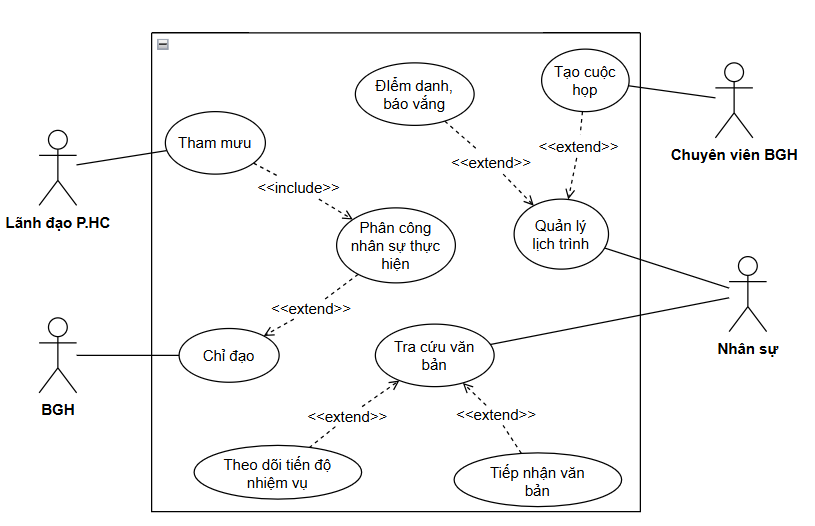
\includegraphics[width=\linewidth]{image/usecase/UC_DOC.png}
    \caption{Sơ đồ Đặc tả Use case nhóm Văn phòng số, nhiệm vụ và lịch công tác}
    \label{fig:uc_ioffice_schedule}
\end{figure}

\usecasespec{
    id={UC-OFF-01},
    name={Phân công xử lý văn bản đến},
    shortname={Phân công văn bản đến},
    actor={Nhân sự được cấp quyền chỉnh sửa phiếu giải quyết văn bản đến},
    desc={Tạo hoặc cập nhật phân công trách nhiệm xử lý văn bản đến trên phiếu giải quyết.},
    pre={Người dùng đã đăng nhập; dữ liệu quyền và trạng thái văn bản cho phép chỉnh sửa phiếu giải quyết.},
    trigger={Người dùng mở màn hình chi tiết văn bản đến và chọn chức năng phân công.},
    mainflow={
            1. Người dùng chọn văn bản đến cần phân công. \newline
            2. Người dùng chọn loại trách nhiệm và đối tượng nhận nhiệm vụ (đơn vị hoặc cá nhân). \newline
            3. Ứng dụng gửi phiếu giải quyết; iOffice tiếp nhận và lưu các phân công hợp lệ, rồi phản hồi kết quả.
        },
    exflow={- iOffice từ chối dữ liệu hoặc không thể lưu: hiển thị lỗi, không xác nhận đã lưu.},
    post={Thông tin phân công được ghi nhận khi iOffice chấp nhận. Phát sinh thông báo phụ thuộc hành động và bước luân chuyển văn bản.},
    label={tab:uc_off_01}
}

\usecasespec{
    id={UC-OFF-02},
    name={Tham mưu văn bản đến},
    shortname={Tham mưu văn bản},
    actor={Lãnh đạo phòng Hành chính},
    desc={Thực hiện tham mưu cho văn bản đến.},
    pre={Người dùng đã đăng nhập, có quyền tham mưu ở bước hiện tại và phiếu giải quyết đã có người chỉ đạo.},
    trigger={Người dùng mở màn hình chi tiết văn bản đến.},
    mainflow={
            1. Người dùng xem chi tiết văn bản đến và các thông tin liên quan. \newline
            2. Người dùng nhập ý kiến và gửi tham mưu. \newline
            3. iOffice ghi nhận ý kiến và xử lý quy trình văn bản theo quyền, trạng thái hiện tại.
        },
    altflow={
            - \textit{1a (Thiếu người chỉ đạo):} Ứng dụng yêu cầu bổ sung người chỉ đạo trên phiếu giải quyết trước khi gửi; người có quyền thực hiện UC-OFF-01.
        },
    post={Ý kiến tham mưu và kết quả xử lý văn bản được iOffice ghi nhận.},
    label={tab:uc_off_02}
}

\usecasespec{
    id={UC-OFF-03},
    name={Chỉ đạo văn bản đến},
    shortname={Chỉ đạo văn bản},
    actor={Ban Giám Hiệu},
    desc={Thực hiện chỉ đạo cho văn bản đến.},
    pre={Ban Giám Hiệu đã đăng nhập và có quyền chỉ đạo cho văn bản đến.},
    trigger={Người dùng mở màn hình chi tiết văn bản đến.},
    mainflow={
            1. Người dùng xem chi tiết văn bản đến và các thông tin liên quan. \newline
            2. Người dùng nhập ý kiến và gửi chỉ đạo. \newline
            3. iOffice ghi nhận ý kiến chỉ đạo và cập nhật quy trình văn bản theo điều kiện hiện tại.
        },
    altflow={
            - \textit{1a (Thực hiện phân công trách nhiệm):} Nếu chưa có thông tin phân công, người dùng tiến hành phân công trách nhiệm (nếu có quyền) (UC-OFF-01). \newline
            - \textit{3a (Nhiệm vụ liên kết):} Khi đã đủ ý kiến chỉ đạo theo phân công, có bước triển khai tiếp theo, văn bản không phải loại thông tin và có người thực hiện, iOffice có thể tạo nhiệm vụ liên kết theo quy trình. \newline
        },
    post={Ý kiến chỉ đạo và kết quả xử lý văn bản được ghi nhận; nhiệm vụ liên kết chỉ phát sinh khi đủ điều kiện quy trình.},
    label={tab:uc_off_03}
}

\usecasespec{
    id={UC-OFF-04},
    name={Tiếp nhận văn bản/nhiệm vụ},
    shortname={Tiếp nhận văn bản},
    actor={Nhân sự được phân công, Lãnh đạo của đơn vị được phân công},
    desc={Ghi nhận việc tiếp nhận văn bản hoặc nhiệm vụ được phân công; phân biệt thao tác tiếp nhận với hoàn thành phần việc được giao.},
    pre={Người dùng đăng nhập và có quyền tiếp nhận văn bản hoặc nhiệm vụ được phân công.},
    trigger={Người dùng mở màn hình chi tiết văn bản đến.},
    mainflow={
            1. Người dùng tiếp nhận văn bản hoặc nhiệm vụ được phân công. \newline
            2. Hệ thống ghi nhận người và thời gian tiếp nhận trên dòng phân công tương ứng. \newline
            3. Hệ thống phản hồi trạng thái tiếp nhận để ứng dụng cập nhật thông tin hiển thị.
        },
    altflow={
            - \textit{2a (Văn bản thông tin hoặc phân công để biết):} Khi tiếp nhận, hệ thống đồng thời ghi nhận hoàn thành dòng phân công tương ứng. \newline
            - \textit{2b (Văn bản giao nhiệm vụ):} Việc tiếp nhận chỉ ghi nhận bắt đầu xử lý, không đồng nghĩa hoàn thành. Sau khi thực hiện công việc, người có quyền sử dụng thao tác \textit{Hoàn thành} riêng trên hệ thống iOffice; hệ thống ghi nhận kết quả hoàn thành theo quy trình. \newline
        },
    post={Dòng phân công được ghi nhận đã tiếp nhận; trạng thái hoàn thành phần việc được ghi nhận ngay ở nhánh thông tin/để biết hoặc sau thao tác hoàn thành riêng đối với văn bản giao nhiệm vụ.},
    label={tab:uc_off_04}
}

\usecasespec{
    id={UC-SCH-01},
    name={Điểm danh hoặc báo vắng cuộc họp},
    shortname={Điểm danh cuộc họp},
    actor={Nhân sự có quyền sử dụng phân hệ lịch, gồm người được phân công và khách tham dự},
    desc={Ghi nhận có mặt, hoàn tác hoặc báo vắng có lý do theo người dùng trong phiên.},
    pre={Người dùng đã đăng nhập, có quyền sử dụng phân hệ lịch; mục lịch tồn tại, chưa bị xóa và có thời gian phù hợp. Đối với luồng trên mobile, người dùng cần mở được chi tiết cuộc họp.},
    trigger={Người dùng mở màn hình chi tiết cuộc họp trên ứng dụng di động.},
    mainflow={
            1. Người dùng mở xem chi tiết cuộc họp trên giao diện Lịch hoặc từ thông báo nhắc việc. \newline
            2. Ứng dụng hiển thị các thao tác điểm danh phù hợp với trạng thái cuộc họp. \newline
            3. Người dùng chọn điểm danh có mặt hoặc báo vắng và nhập lý do khi cần. \newline
            4. Ứng dụng gửi yêu cầu; iOffice kiểm tra phiên, quyền phân hệ lịch, sự tồn tại của mục lịch, thời gian và trạng thái tham dự hiện tại. \newline
            5. iOffice ghi nhận theo dòng phân công nếu có; nếu không, ghi nhận khách tự điểm danh riêng. Ứng dụng cập nhật trạng thái tham dự từ phản hồi.
        },
    altflow={
            - \textit{Luồng 3a (Đổi trạng thái):} Người đã báo vắng có thể chuyển sang có mặt trong khung giờ điểm danh hợp lệ. \newline
            - \textit{Luồng 3b (Hoàn tác):} Người đã điểm danh có mặt có thể hoàn tác trong khung giờ cho phép rồi thực hiện lại thao tác phù hợp.
        },
    exflow={
            - \textit{Ngoại lệ 4a (Ngoài khung thời gian):} Thao tác thực hiện ngoài khung giờ quy định $\rightarrow$ hệ thống từ chối và thông báo lý do. \newline
            - \textit{Ngoại lệ 4b (Không đủ quyền phân hệ, phiên không hợp lệ hoặc lịch đã xóa):} iOffice từ chối yêu cầu. \newline
            - \textit{Ngoại lệ 4c (Thiếu lý do hoặc đã có mặt):} Báo vắng phải có lý do hợp lệ; thao tác điểm danh lại khi đã có mặt bị từ chối.
        },
    post={Trạng thái tham dự được ghi nhận và kết quả mới được phản hồi trên ứng dụng.},
    label={tab:uc_sch_01}
}

\usecasespec{
    id={UC-SCH-02},
    name={Xem lịch làm việc tổng hợp},
    shortname={Xem lịch tổng hợp},
    actor={Nhân sự},
    desc={Cho phép người dùng theo dõi lịch họp iOffice, lịch nghỉ phép HRM và lịch công tác HRM trên một giao diện tuần duy nhất.},
    pre={Người dùng đã đăng nhập và có quyền truy cập dữ liệu nguồn tương ứng.},
    trigger={Người dùng mở mục ``Lịch biểu'' trên ứng dụng di động.},
    mainflow={
            1. Người dùng mở mục ``Lịch biểu'' trên ứng dụng. \newline
            2. Ứng dụng tải lịch iOffice và các dữ liệu nghỉ phép, công tác HRM được phép truy cập trong khoảng thời gian cần xem. \newline
            3. Ứng dụng hiển thị các sự kiện trên giao diện lịch tuần thống nhất, phân biệt rõ nguồn dữ liệu qua màu sắc và nhãn phân loại. \newline
            4. Người dùng chọn một sự kiện cụ thể để xem chi tiết hoặc chuyển đến màn hình nghiệp vụ liên quan.
        },
    exflow={
            - \textit{Ngoại lệ 2a (Lỗi tải lịch):} Khi có lỗi được truyền đến giao diện, ứng dụng hiển thị lỗi và cho phép tải lại. Yêu cầu xử lý lỗi từng nguồn được nêu ở NFR-01; mức đáp ứng hiện tại được đối chiếu tại Chương~6.
        },
    post={Các sự kiện tải được hiển thị trên lịch tổng hợp; việc tra cứu không thay đổi dữ liệu nguồn.},
    label={tab:uc_sch_02}
}

Điểm danh có mặt và hoàn tác được thực hiện từ một giờ trước giờ bắt đầu đến hết ngày kết thúc cuộc họp. Báo vắng được thực hiện đến hết ngày bắt đầu, với lý do từ 1 đến 200 ký tự sau khi loại khoảng trắng đầu/cuối. Chuyển từ vắng sang có mặt tuân theo cửa sổ điểm danh. Thẻ thống kê đếm các dòng phân công; khách được hiển thị ở nhóm riêng, không cộng vào tổng này.

\subsubsection{Tạo và đăng ký cuộc họp}

\usecasespec{
 id={UC-SCH-03}, name={Tạo và đăng ký cuộc họp}, shortname={Tạo cuộc họp},
 actor={Chuyên viên BGH được cấp quyền đối với tạo trực tiếp Trường; nhân sự có quyền tương ứng đối với các nhánh khác},
 desc={Chuẩn bị và lưu thông tin cuộc họp bằng biểu mẫu native, lựa chọn nhánh theo quyền do iOffice cung cấp.},
 pre={Người dùng đăng nhập, có quyền sử dụng lịch và quyền của nhánh được chọn; danh mục, quy trình đang hoạt động đáp ứng yêu cầu backend.},
 trigger={Người dùng chọn Tạo lịch trên màn hình Lịch biểu.},
 mainflow={1. Ứng dụng hiển thị các lựa chọn tạo được tài khoản cho phép. \newline
 2. Chuyên viên BGH chọn tạo trực tiếp lịch Trường. \newline
 3. Người dùng nhập tiêu đề, loại lịch, thời gian, địa điểm và ghi chú; chọn chủ trì, người tham dự, thư ký và tệp theo quyền. \newline
 4. Ứng dụng kiểm tra biểu mẫu, gửi yêu cầu tạo tới iOffice. \newline
 5. iOffice kiểm tra quyền và thành phần; lịch Trường cần ít nhất một phân công thuộc BGH, HĐT hoặc VPĐU. Người tạo và đơn vị tạo được xác định từ phiên; lịch lưu ở bước tổng hợp cùng các phân công hợp lệ. \newline
 6. Hệ thống kích hoạt cơ chế gửi lời mời của bản demo sau khi lưu và trả kết quả; bước này không xác nhận thiết bị đã nhận thông báo. \newline
 7. Ứng dụng tải các tệp đã chọn bằng yêu cầu riêng rồi làm mới lịch; người tạo xem trạng thái chưa phát hành.},
 altflow={- Nhánh đơn vị: lưu theo hợp đồng lịch đơn vị. \newline
 - Nhánh đăng ký Trường: tạo phiếu đăng ký, lưu mục/tệp rồi gửi phiếu theo quy trình; không đồng nhất với tạo trực tiếp.},
 exflow={- Dữ liệu chưa hợp lệ hoặc thiếu thành phần bắt buộc của lịch Trường: yêu cầu bổ sung; backend có thể trả thông báo lỗi chung. \newline
 - Không đủ quyền, hết phiên hoặc lỗi lưu: backend từ chối, ứng dụng không thông báo đã tạo. \newline
 - Đã nhận ID nhưng upload lỗi: mục lịch có thể đã tồn tại; ứng dụng giữ ID và phần tệp đã tải trong phiên form để thử lại trên mục đó. \newline
 - Mất phản hồi tạo: kết quả có thể chưa xác định; không có bảo đảm chống trùng tuyệt đối khi tạo lại.},
 post={Với nhánh trực tiếp thành công, mục lịch có người tạo, phân công và trạng thái tổng hợp; tệp được ghi nhận khi upload thành công. Lịch chưa được coi là phát hành chính thức.}, label={tab:uc_sch_03}
}

\begin{table}[H]
\centering\small
\caption{Các nhánh tạo và đăng ký lịch}\label{tab:schedule_create_permissions}
\begin{tabularx}{\textwidth}{|L{3.5cm}|Y|}\hline
\textbf{Nhánh} & \textbf{Ý nghĩa} \\\hline
Đơn vị & Lập lịch họp nội bộ của đơn vị. \\\hline
Đăng ký Trường & Lập và gửi phiếu đăng ký để được tiếp nhận theo quy trình. \\\hline
Trực tiếp Trường & Lưu lịch họp cấp Trường ở bước tổng hợp, chưa phát hành chính thức. \\\hline
\end{tabularx}
\end{table}

Các lựa chọn tạo lịch được hiển thị theo quyền tài khoản. Với nhánh tạo trực tiếp cấp Trường, lịch được lưu ở bước tổng hợp để tiếp tục xử lý, chưa phải lịch chính thức đã phát hành.

Thiết kế chức năng tạo lịch được trình bày tại Mục~\ref{subsec:create_schedule_integration}.

\subsubsection{Biểu đồ hoạt động}
\subsubsubsection{Quy trình điểm danh và báo vắng cuộc họp}

Hình~\ref{fig:act_attendance} minh họa quy trình điểm danh và báo vắng của người được phân công. Nhánh khách và khung thời gian được mô tả tại UC-SCH-01 và biểu đồ tuần tự.

\begin{figure}[H]
    \centering
    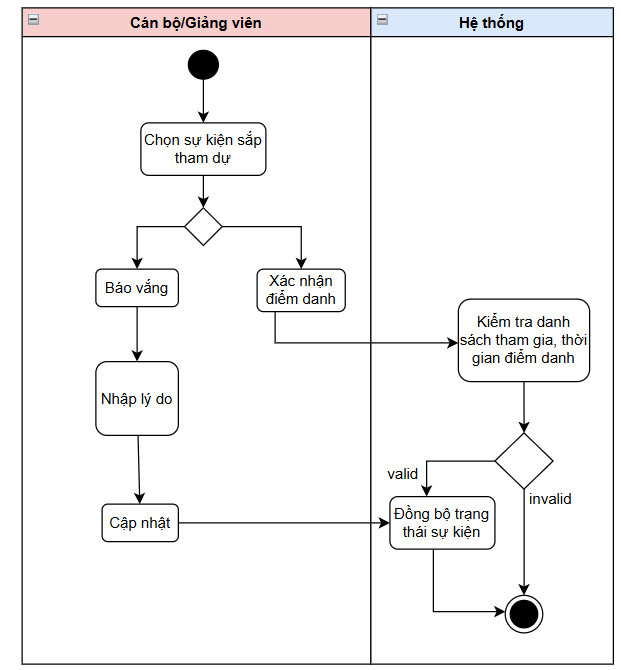
\includegraphics[width=0.95\linewidth]{image/uml/attendant_activity.png}
    \caption{Biểu đồ hoạt động Điểm danh và báo vắng cuộc họp của người được phân công}
    \label{fig:act_attendance}
\end{figure}

\subsubsubsection{Quy trình xử lý văn bản đến}
Hình~\ref{fig:ID_ACT} thể hiện luân chuyển văn bản đến qua các bước xử lý.

\begin{figure}[H]
    \centering
    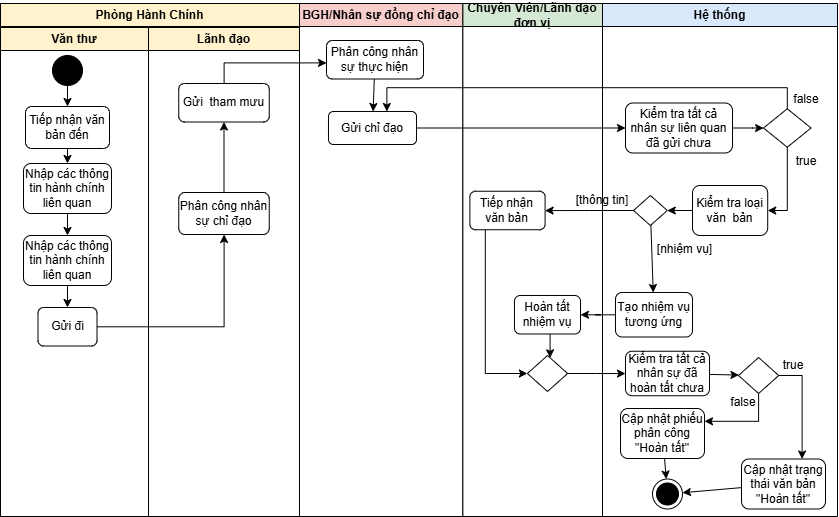
\includegraphics[width=\linewidth]{image/uml/doc_activity.png}
    \caption{Sơ đồ hoạt động: Văn bản đến}
    \label{fig:ID_ACT}
\end{figure}

\subsubsection{Biểu đồ tuần tự}

\subsubsubsection{Điểm danh và báo vắng cuộc họp}

Hình~\ref{fig:seq_attendance} thể hiện kiểm tra điều kiện, ghi nhận theo phân công hoặc khách và cập nhật kết quả của UC-SCH-01.

\begin{figure}[H]
    \centering
    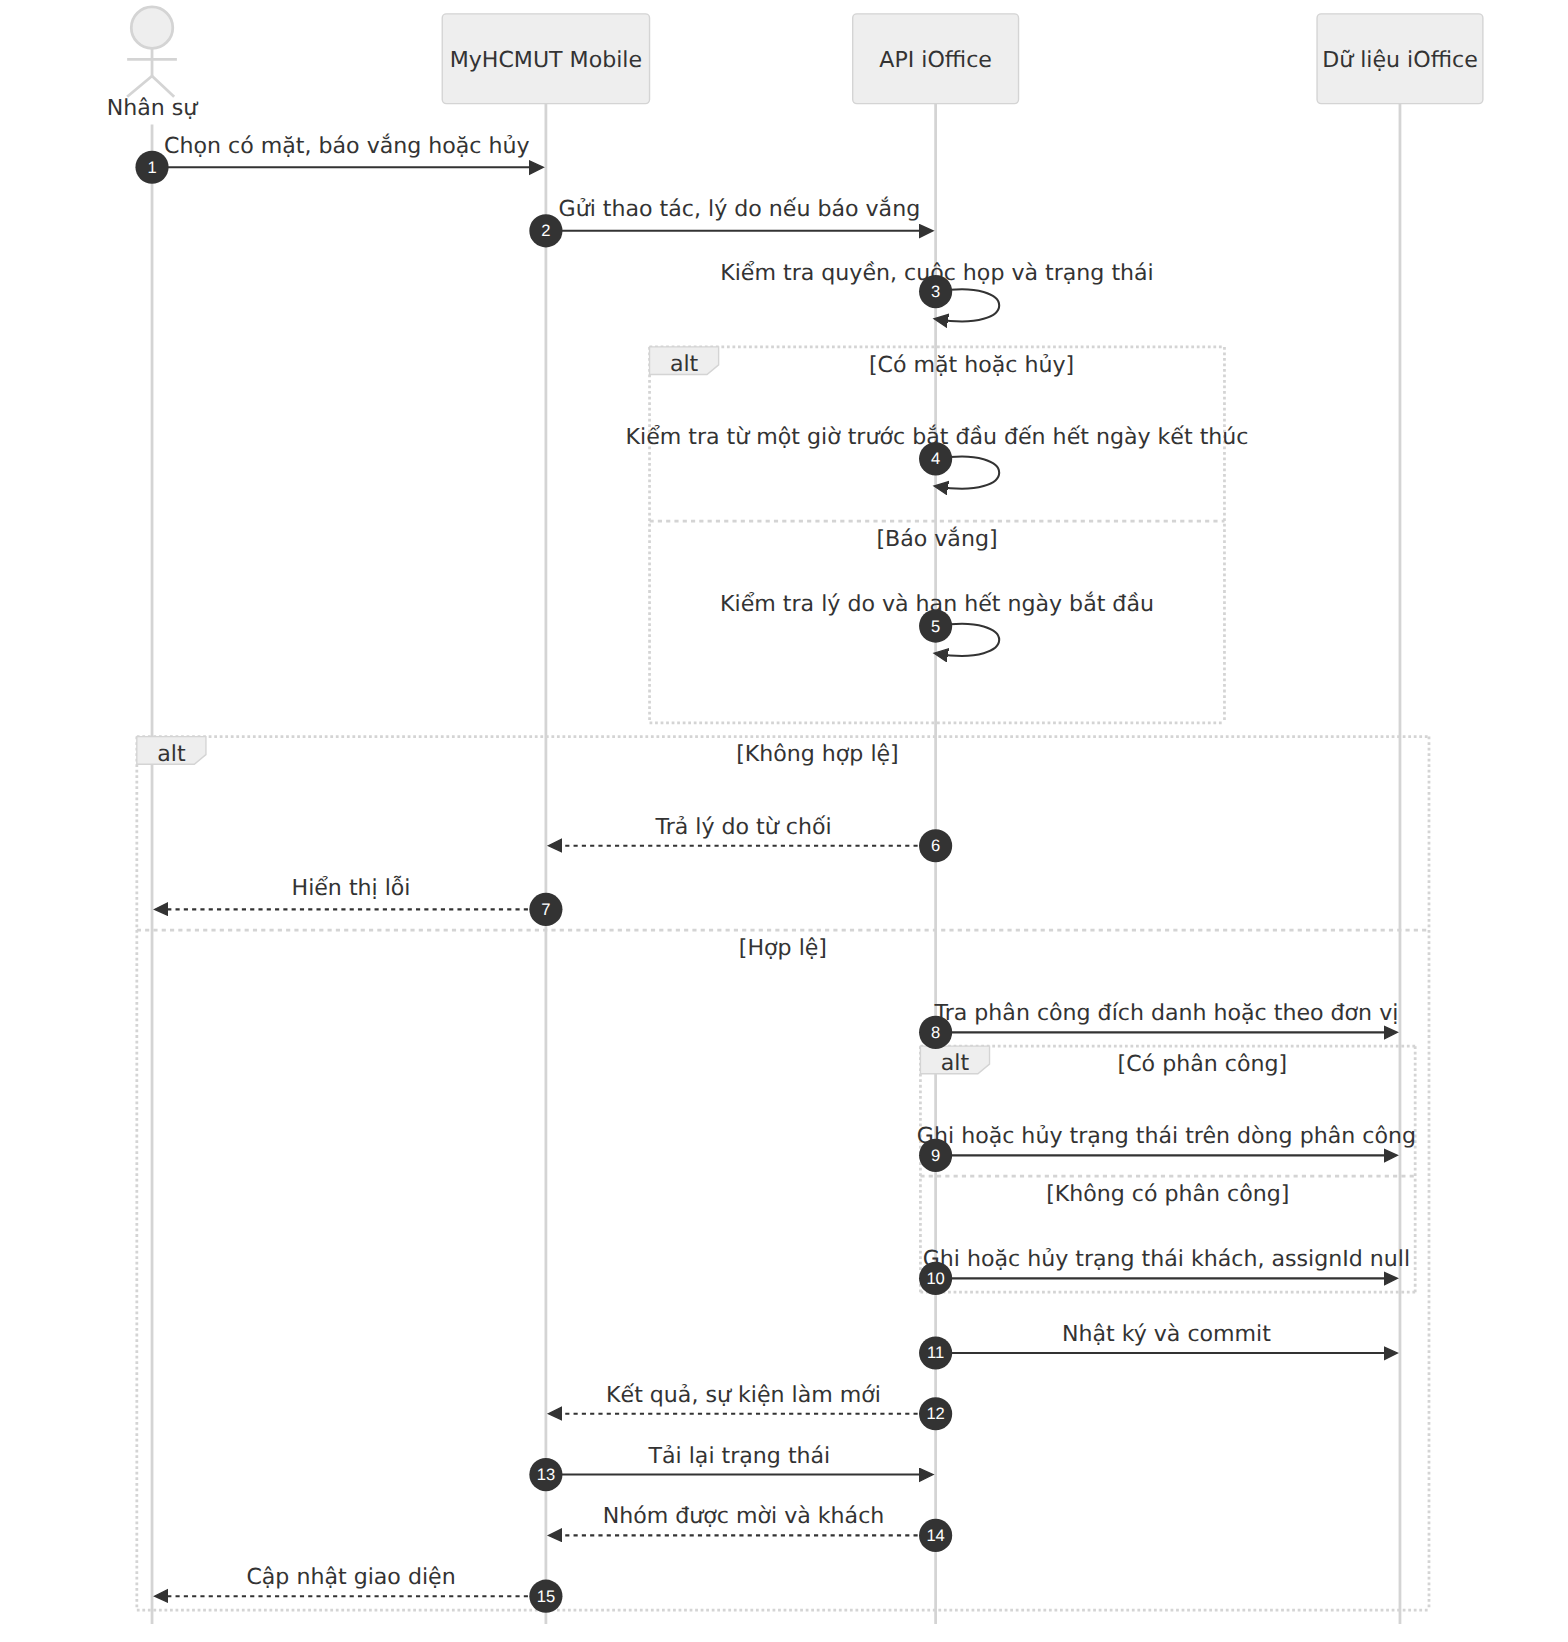
\includegraphics[width=\linewidth]{image/uml/seq_attendance.png}
    \caption{Biểu đồ tuần tự Điểm danh và báo vắng cuộc họp}
    \label{fig:seq_attendance}
\end{figure}

\subsubsubsection{Tạo trực tiếp lịch họp cấp Trường}

Hình~\ref{fig:schedule_create_integration} thể hiện lưu lịch ở tổng hợp và bổ sung tài liệu sau đó. Lỗi tải tài liệu không làm mất lịch đã lưu; tạo trực tiếp chưa phải phát hành lịch chính thức.

\begin{figure}[H]
    \centering
    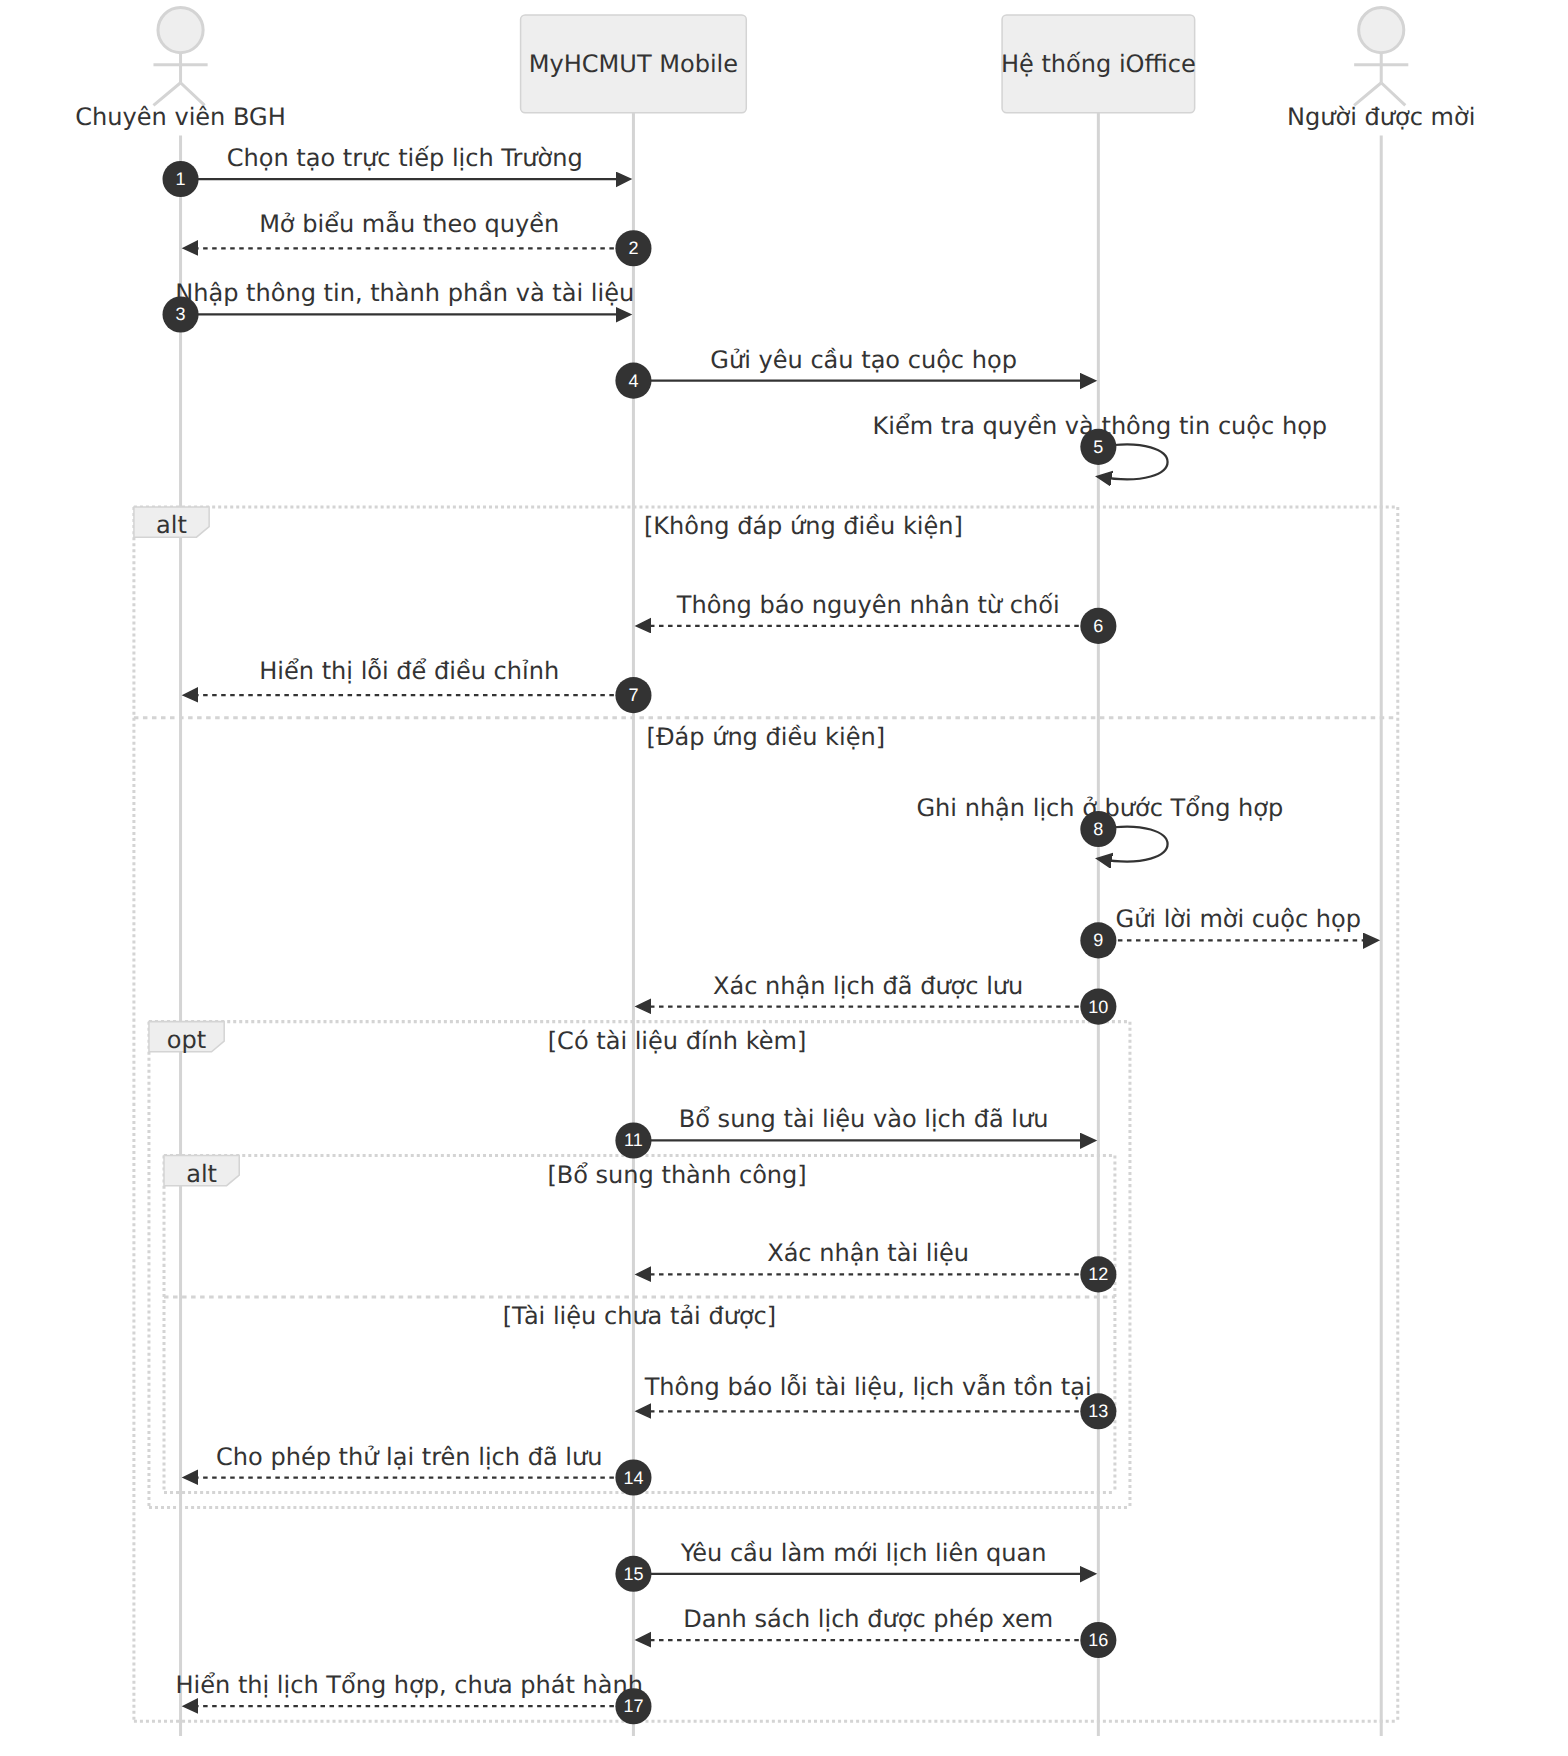
\includegraphics[width=\linewidth,height=0.66\textheight,keepaspectratio]{image/uml/seq_schedule_create.png}
    \caption{Biểu đồ tuần tự nghiệp vụ tạo trực tiếp lịch họp cấp Trường}
    \label{fig:schedule_create_integration}
\end{figure}
% END SOURCE: Chapter4/section2/ioffice_schedule/index.tex

% END SOURCE: Chapter4/section2/index.tex

\newpage

% BEGIN SOURCE: Chapter4/section3.tex
\section{Yêu cầu phi chức năng}
\label{sec:yeucau_phichucnang}

Các yêu cầu phi chức năng xác định những mục tiêu chất lượng cần xem xét trong quá trình thiết kế và hiện thực MyHCMUT Mobile. Mức độ đáp ứng được đánh giá thông qua kết quả kiểm thử và các giới hạn trình bày tại Chương~6.

\begin{table}[H]
\centering\small
\caption{Yêu cầu phi chức năng của MyHCMUT Mobile}
\label{tab:nfr}
\begin{tabularx}{\textwidth}{|L{1.8cm}|L{3.4cm}|Y|}
\hline
\textbf{Mã} & \textbf{Yêu cầu} & \textbf{Nội dung đặc tả} \\
\hline
NFR-01 & Tính ổn định & Cần xử lý mất kết nối, quá thời gian chờ và lỗi hệ thống nguồn. Cần phân biệt dữ liệu rỗng với dữ liệu chưa tải được; chỉ báo thao tác thành công sau xác nhận của backend. \\
\hline
NFR-02 & Khả năng sử dụng & Giao diện cần nhất quán, phù hợp thao tác di động; biểu mẫu nhiều thông tin được chia bước. Cần thể hiện trạng thái tải, lỗi, kết quả và điều kiện tiếp tục thao tác. \\
\hline
NFR-03 & Bảo mật và phân quyền & Cần xác thực trước khi truy cập nghiệp vụ. UI phản ánh quyền tài khoản; backend cần kiểm tra quyền theo nghiệp vụ, đối tượng và bước xử lý, kể cả yêu cầu gọi trực tiếp. \\
\hline
NFR-04 & Tính nhất quán dữ liệu & Dữ liệu chính thức do hệ thống nguồn quản lý; dữ liệu cục bộ chỉ hỗ trợ sử dụng. Sau thao tác ghi, cần phản ánh kết quả được backend ghi nhận; kết quả chưa xác định khi mất phản hồi không được coi là lưu thất bại chắc chắn. \\
\hline
NFR-05 & Khả năng bảo trì và mở rộng & Mục tiêu thiết kế là tổ chức mã theo nhóm nghiệp vụ và tách thành phần dùng chung, hạn chế phụ thuộc không cần thiết để hỗ trợ thay đổi và kiểm thử. \\
\hline
\end{tabularx}
\end{table}

Các yêu cầu trên được dùng làm tiêu chí đối chiếu khi đánh giá hệ thống. Kết quả đánh giá và các giới hạn tương ứng được trình bày tại Chương~6.

\section{Kết luận chương}
\label{sec:ketluan_chuong4}

Chương này đã xác định các nhóm người dùng, yêu cầu chức năng và yêu cầu phi chức năng của MyHCMUT Mobile. Các yêu cầu chức năng được phân tích theo những nhóm nghiệp vụ chính và được làm rõ thông qua các ca sử dụng, biểu đồ hoạt động và biểu đồ tuần tự đối với các quy trình quan trọng. Bên cạnh đó, các yêu cầu phi chức năng xác định những yêu cầu về tính ổn định, khả năng sử dụng, bảo mật và phân quyền, tính nhất quán dữ liệu, cũng như khả năng bảo trì và mở rộng của ứng dụng.

Các yêu cầu được xác định trong chương này là cơ sở cho việc thiết kế kiến trúc, tổ chức các thành phần ứng dụng và xây dựng các cơ chế tích hợp với hệ thống nghiệp vụ hiện hữu được trình bày trong Chương 5.
% END SOURCE: Chapter4/section3.tex
% END SOURCE: Chapter4/index.tex
